\documentclass[a4paper,openright,12pt]{book}
\usepackage{graphicx}
% \usepackage[sort&compress]{natbib}
\usepackage[spanish]{babel}
\usepackage{epsfig}
\usepackage{rotating}
\usepackage{amsmath}
\usepackage{slashbox}
\usepackage{setspace}
\usepackage{amsfonts}
\usepackage{dcolumn}
\usepackage{multirow}
\usepackage{url}
%\usepackage{natbib}
\usepackage{amssymb}
\usepackage{times}
\usepackage{fontspec}
\usepackage{booktabs}
\usepackage{geometry}
\usepackage{cite}
\usepackage{caption}
% \usepackage[utf8]{inputenc}

\setcounter{secnumdepth}{3}
\setmainfont{Times New Roman}
\geometry{left=3cm,right=3cm,top=2.5cm,bottom=2.5cm}

\RequirePackage{ifpdf} % ¿latex o pdflatex?
% Configuración de las imágenes

\usepackage{graphicx}		% Inclusión de imágenes
\DeclareGraphicsExtensions{.pdf}

\graphicspath{ {../imgs/} } % Ruta respecto al fichero tex principal dónde se buscan imágenes

\onehalfspace
\begin{document}

% ---------------- pagina de presentación: portada --------------------------
\pagestyle{empty}
\begin{titlepage}

\begin{center}
\vspace*{-1in}
\begin{figure}[htb]
\begin{center}

\includegraphics[height=2cm]{logo_uz}
\hfill
\includegraphics[height=2cm]{logo_fecem}
\end{center}
\end{figure}
\vspace*{0.15in}
FACULTAD DE CIENCIAS ECONÓMICAS Y EMPRESARIALES \\
\vspace*{0.15in}
DEPARTAMENTO DE ESTRUCTURA ECONÓMICA\\
\vspace*{0.6in}
\begin{large}
TRABAJO\\
\end{large}
\vspace*{0.2in}
\begin{Large}
\textbf{COMERCIO INTERNACIONAL} \\
\end{Large}
\vspace*{0.3in}
\begin{large}
Análisis De La Economía De Chipre \\ 
\end{large}
\vspace*{0.3in}
%\rule{80mm}{0.1mm}\\
%\vspace*{0.1in}
\begin{large}
Autor: \\
Maximiliano Greco \\
\end{large}
\end{center}

\end{titlepage}

\newpage


% -------------- EMPIEZA LA READACCIÓN-----------------------------------------

\chapter{Presentación Del País}
\label{cap1}


\section{Situación Geográfica}


\begin{figure}[htb]
    \centering
    \caption{Situación geográfica de Chipre.}
    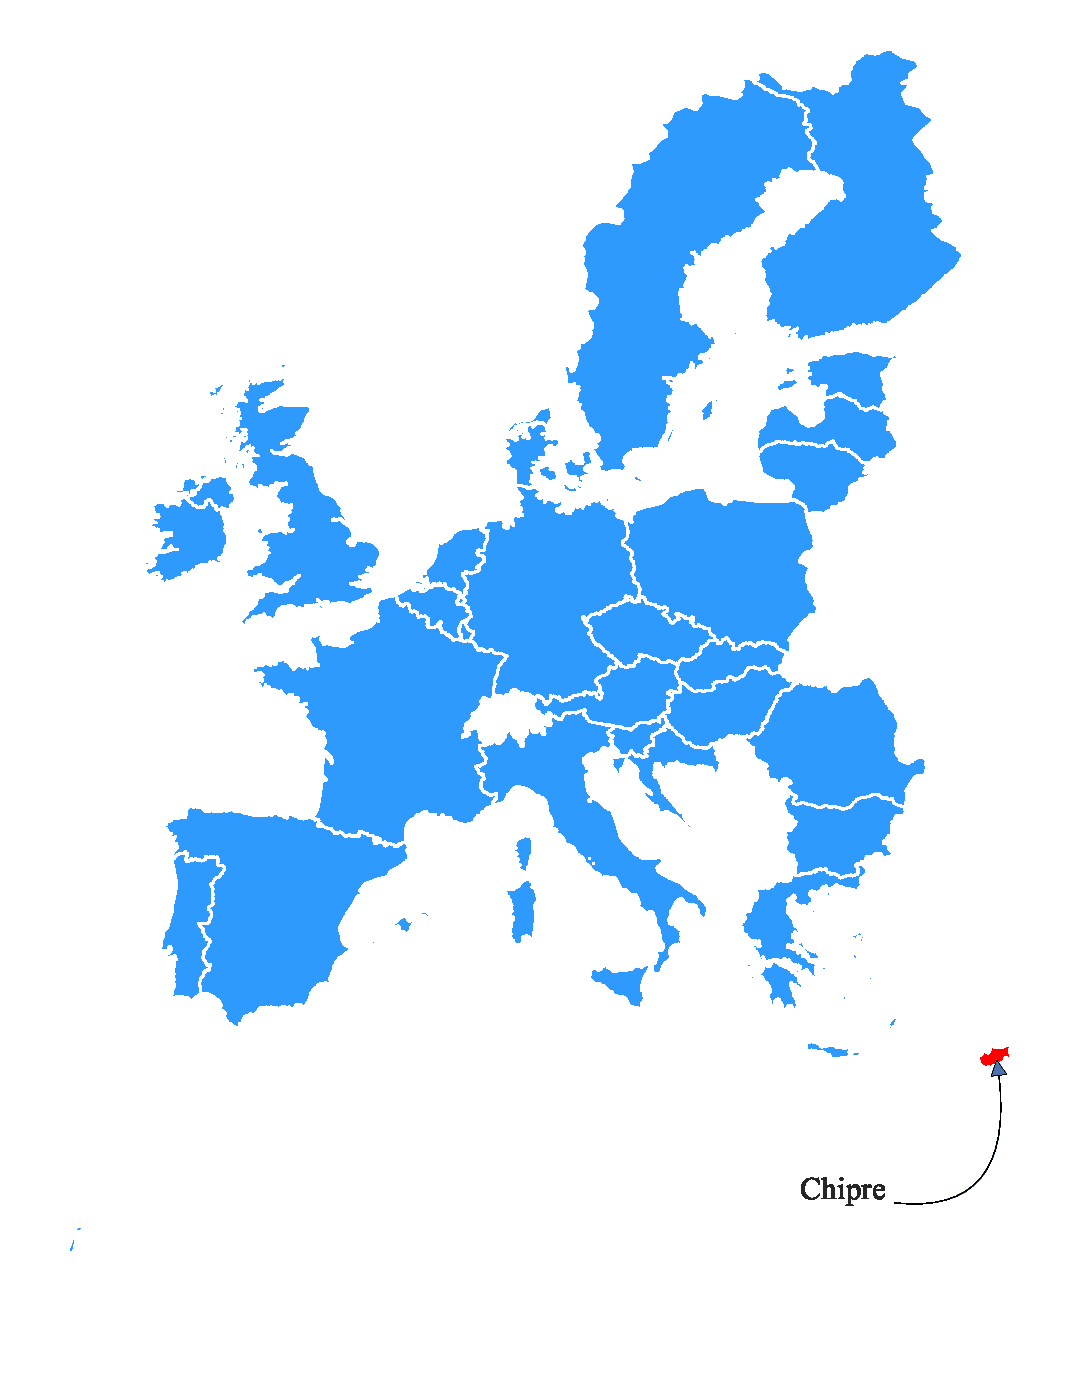
\includegraphics[width=9cm]{mapa}
    \caption*{\textit{Fuente}: Elaboración propia a partir de Shapefile de Eurostat}
    \label{fig1}
\end{figure}

\section{Historia}

Chipre no así como su tamaño, posee una gran riqueza cultural e histórica, ya en la prehistoria disponía de pozos de agua, los más antiguos del mundo[cita], hasta poblados del neolítico[cita]. Chipre ha albergado a diversas culturas, cómo la Griega y la fenicia (Antigua región originalmente que en la actualidad iba desde Israel hasta Siria), pasando por Egipcios, persas, el imperio romano, Bizantino (actual Turquía), Árabe, Rep. de Venecia, Turco-Otomana, británica y griega otra vez.\cite{ChipreWi15:online}

En 1974 se produce un golpe de estado por el gobierno Turco, invadiendo el tercio norte de Chipre, y dando origen a la Rep. Turca del Norte de Chipre (RTNC) formando un estado que sólo reconoce Turquía e ignorado por la comunidad internacional. En 2004 Chipre entra en la Unión Europea. \cite{ICEXEspa12:online}

Chipre se divide en seis distritos:

\begin{enumerate}
    \item Nicosia: Se encuentra en la RTNC
    \item Famagusta: Se encuentra en la RTNC
    \item Limassol
    \item Pafos
    \item Lárnaca
    \item Kyrenia: Se encuentra en la RTNC
\end{enumerate}

 Además, en el sur existen dos territorios que son bases militares bajo el mando de Reino Unido.

\begin{enumerate}
    \item Acrotiri
    \item Dhekelia
\end{enumerate}

\begin{figure}[ht]
    \centering
    \caption{Distritos de Chipre}
    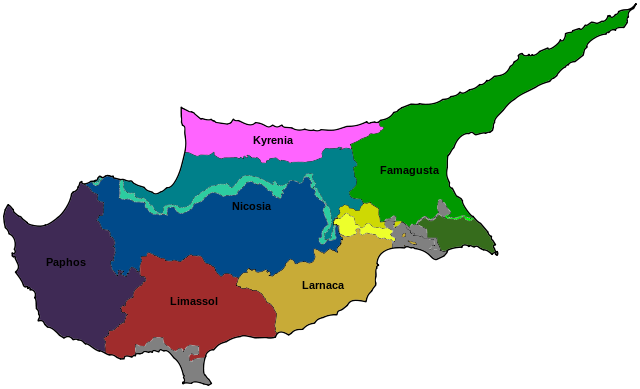
\includegraphics[width=9cm]{mapa_distritos.png}
    \caption*{\textit{Fuente}: \cite{ChipreWi33}}
    \label{mapdistrics}
\end{figure}

% --------------------------------------- RECURSOS NATURALES ------------------

\section{Recursos Naturales}

Recursos Naturales de Chipre:
Según el ICEX, los recursos naturales que dispone Chipre, se encuentran listados a continuación:

\begin{enumerate}
    \item Cobre
    \item Pirita
    \item Asbesto
    \item Yeso
    \item Madera
    \item Sal
    \item Mármol
    \item Tierra de arcilla.
    \item Gas natural
    \item Petróleo
\end{enumerate}

\*Actualmente se encuentra en fase de exploración y análisis para su futura explotación que se estima a partir 2018-2020.

Fuente: ICEXEspa50

% -------------------------------------  GRUPO ECONOMICOS -------------------
\section{Grupos Económicos}

Cuadro de organizaciones internacionales económicas y comerciales de la que el país es miembro \cite{ICEXchipreGrupos:online}:

% resetear numeación

\begin{enumerate}
    \item La Organización de Naciones Unidas (1960).
    \item El Consejo de Europa (1961).
    \item La Commonwealth (1961).
    \item El Fondo Monetario Internacional (1962).
    \item El Banco Mundial (1962).
    \item La Organización para la Seguridad y la Cooperación en Europa (O.S.C.E.) (1975).                               
    \item Organización Marítima Internacional (1978).
    \item La Organización Mundial del Comercio (1995).
    \item La Unión Europea (desde el 1 de mayo de 2004) y la Eurozona (2008).
\end{enumerate}

% -------------------------------- INSTITUCIONES INTERNACIONALES -------------

\section{Instituciones Internacionales}

\textbf{Resumen de las relaciones económicas internacionales} \cite{ICEXChipre96:online}

La Unión Europea es el principal socio comercial de Chipre (44,21\% de las exportaciones y el 71,32\% de las importaciones en 2014).

\textbf{FMI}


La República de Chipre ingresó en el FMI el 21 de diciembre 1961. El 25 de Junio de 2012 el país paso a ser   el quinto socio europeo en solicitar ayuda financiera al Fondo Monetario Internacional.

\textbf{Banco Mundial y entidades asociadas}

Chipre no es beneficiaria de préstamo alguno por parte del Banco Mundial.
 Pertenece al Banco Internacional de Reconstrucción y Desarrollo (BIRD) desde el 21 de diciembre 1961. Chipre no es beneficiario de préstamo alguno procedente del mismo. 
En el ámbito privado, durante el año 1983 y el año 1991 fue beneficiaria de sendos préstamos de la Corporación Financiera Internacional (IFC) dirigidos al sector de la hostelería y el turismo.
Pertenece al ICSID (International Centre for Settlement of Investment Disputes), desde el año 1966.

\textbf{Con la Organización Mundial de Comercio}

La República de Chipre pertenecía al GATT desde el 15 de julio 1963. La entrada en vigor de la OMC adelanto  la eliminación de las restricciones cuantitativas  dando lugar a una mayor previsibilidad,  en especial con la consolidación de la mayoría de los aranceles (Chipre es miembro de la OMC desde el 30 de Julio de 1995). Además, Chipre adoptó el Arancel Común Exterior de la UE (para productos procedentes de terceros países) en Enero 1998, y pertenece a la UE desde el 1 de Mayo 2004 (los Estados Miembros de la UE son Miembros de la OMC por derecho propio).Con otros Organismos y Asociaciones

\textbf{Chipre y las Naciones Unidas}


Chipre desde el 20 de septiembre de 1960 es miembro de las Naciones Unidas. . A través de su participación y pertenencia a los órganos de la ONU. Chipre y el Consejo de Europa

Chipre ha sido miembro del Consejo de Europa desde su independencia. Desde su adhesión en mayo de 1961, Chipre ha participado activamente en todos los organismos y órganos del Consejo, incluida la Asamblea Parlamentaria. 

\textbf{Chipre y la Organización Marítima Internacional}

Chipre es miembro de la Organización Marítima Internacional (OMI) desde 1978. 

\textbf{Chipre y la Commonwealth}


La República de Chipre se convirtió en miembro de la COMMONWEALTH en el año 1961.

\section{Rasgos Económicos}

\subsection{Importancia económica del país en la región}

Debido a su ubicación  o las principales relaciones comerciales que mantiene el país,  podemos comparar Chipre con países como Egipto, Siria, Turquía y Grecia.
Chipre es el país más pequeño por extensión y, consecuentemente, por población y PIB. Se encuentra dentro de los países de inflación moderada no obstante con un alto déficit por cuenta corriente en relación con el PIB. Sin embargo, a pesar de estas limitaciones, su ubicación geográfica, sus recursos agrícolas, forestales y minerales, y especialmente las reservas de gas natural recientemente descubiertas, atribuyen al país una gran importancia estratégica. 
Podemos decir que Chipre se encuentra en medio de una serie de países pequeños que no tienen una oferta exportadora de bienes relevante, por lo que cada uno de ellos tiene que recurrir a una fórmula diferente para financiar su sector exterior. Ésta sería, en el caso de Chipre, en una pequeña parte los fletes y, principalmente, el turismo y las inversiones atraídas por su situación como centro financiero de dos zonas con problemas: los países ex-comunistas y Oriente Medio\cite{ICEXChipre18:online}.

\subsection{Marco institucional de la Política Comercial con la Unión Europea}

Peso de Chipre en el comercio de la UE. Chipre es miembro de la UE desde el 1 de mayo de 2004 y adoptó el euro el 1 de enero de 2008. Chipre comercia con sus socios comunitarios más que la media de la UE aunque el peso de Chipre en el comercio extra-comunitario es muy reducido.
Posición en la Ronda de Doha. Chipre apoya la conclusión de estas negociaciones aunque muestra preocupación acerca de una propuesta para la liberalización completa del tránsito, presentada por Turquía.
Relaciones bilaterales. Chipre apoya la negociación de acuerdos comerciales bilaterales. en especial por la necesidad de tener seguridad jurídica y proteger a los inversores.
Otras cuestiones destacables. En general, Chipre mantiene posiciones bastante liberales ya que necesita crucialmente del comercio por su condición de pequeña isla\cite{ICEXEspa63:online}.


\section{Sectores Releevantes En La Produción Y Comercio Exterior}
La principal fuente de ingresos de Chipre se produce en el sector servicios, y especialmente del turismo del cual obtiene un 40\% de los ingresos anuales\cite{OMCExamen}.

\subsection{Principales socios comerciales (exportación e importación)}

El principal destino de las exportaciones es la Unión Europea. Los 7 destinos principales de la exportación chipriota en el año 2015 han sido\cite{OMCExamen} \cite{ICEXChipre96:online}:

\begin{enumerate}
    \item Grecia
    \item Irlanda
    \item Reino Unido
    \item Israel
    \item Arabia Saudí
    \item Egipto
    \item Líbano.
    \item España representó el 0,38\% del total de las exportaciones en este año. 
\end{enumerate}

La mayor parte de las transacciones se realizan con países miembros de la UE-28. Principales productos exportados e importados. La dependencia de Chipre de combustibles supone que el capítulo “Combustibles, aceites minerales” sea el más significativo de cada año. Éste supuso en 2015 un 22,42\% de las importaciones totales\cite{ICEXEspa16:online}.

\section{Relación Real de Intercambio}

La relación real de intercambio (RRI) se define cómo $RRI = \frac{P_x}{P_m} = \frac{IVU_x}{IVU_m} 100$ \cite{krugman2015international}  por tanto, cuando la relación real de intercambio es mayor (menor) que 100, implica que el valor de las exportaciones son mayores (menores) que el valor de las importaciones, por lo que para una misma cantidad de exportaciones el país puede obtener una mayor (menor) cantidad de importaciones, lo cual mejora (empeora) el bienestar, y por consiguiente , el comercio internacional reporta beneficios (pérdidas) para el país en cuestión.

\begin{table}[]
    \centering
    \caption{Relación real de intercambio}
    \label{tab_rri}
    \resizebox{\textwidth}{!}{%
    \begin{tabular}{@{}lllllllllllll@{}}
    \toprule
    AÑO                                                 & 2003     & 2004     & 2005     & 2006     & 2007     & 2008     & 2009     & 2010     & 2011     & 2012     & 2013     & 2014     \\ \midrule
    Exportaciones de bienes y servicios (corriente LCU) & 7,42E+09 & 7,88E+09 & 8,25E+09 & 8,55E+09 & 9,33E+09 & 9,42E+09 & 8,72E+09 & 9,10E+09 & 9,65E+09 & 9,65E+09 & 9,21E+09 & 9,70E+09 \\
    Exportaciones de bienes y servicios (constante LCU) & 7,89E+09 & 8,09E+09 & 8,25E+09 & 8,36E+09 & 8,80E+09 & 8,65E+09 & 8,02E+09 & 8,23E+09 & 8,58E+09 & 8,43E+09 & 8,01E+09 & 8,47E+09 \\
    Importaciones de bienes y servicios (corriente LCU) & 7,22E+09 & 7,90E+09 & 8,33E+09 & 9,02E+09 & 1,02E+10 & 1,14E+10 & 9,55E+09 & 1,02E+10 & 1,03E+10 & 1,00E+10 & 8,76E+09 & 9,22E+09 \\
    Importaciones de bienes y servicios (constante LCU) & 7,67E+09 & 8,21E+09 & 8,33E+09 & 8,81E+09 & 9,73E+09 & 1,05E+10 & 8,80E+09 & 9,20E+09 & 9,14E+09 & 8,72E+09 & 7,54E+09 & 8,14E+09 \\
    IVUX                                                & 94,01    & 97,45    & 100,00   & 102,28   & 105,97   & 108,88   & 108,75   & 110,51   & 112,54   & 114,45   & 114,92   & 114,54   \\
    IVUM                                                & 94,17    & 96,28    & 100,00   & 102,39   & 104,41   & 109,12   & 108,51   & 110,42   & 112,87   & 114,97   & 116,25   & 113,23   \\
    RRI                                                 & 99,84    & 101,21   & 100,00   & 99,89    & 101,50   & 99,78    & 100,22   & 100,08   & 99,71    & 99,54    & 98,86    & 101,16   \\ \bottomrule

    \end{tabular}}
    \caption*{\textit{Fuente}: Elaboración propia con datos de \textit{World Bank API (WDI)}}
\end{table}

\begin{figure}[ht]
    \centering
    \caption{Relación Real de Intercambio de Chipre}
    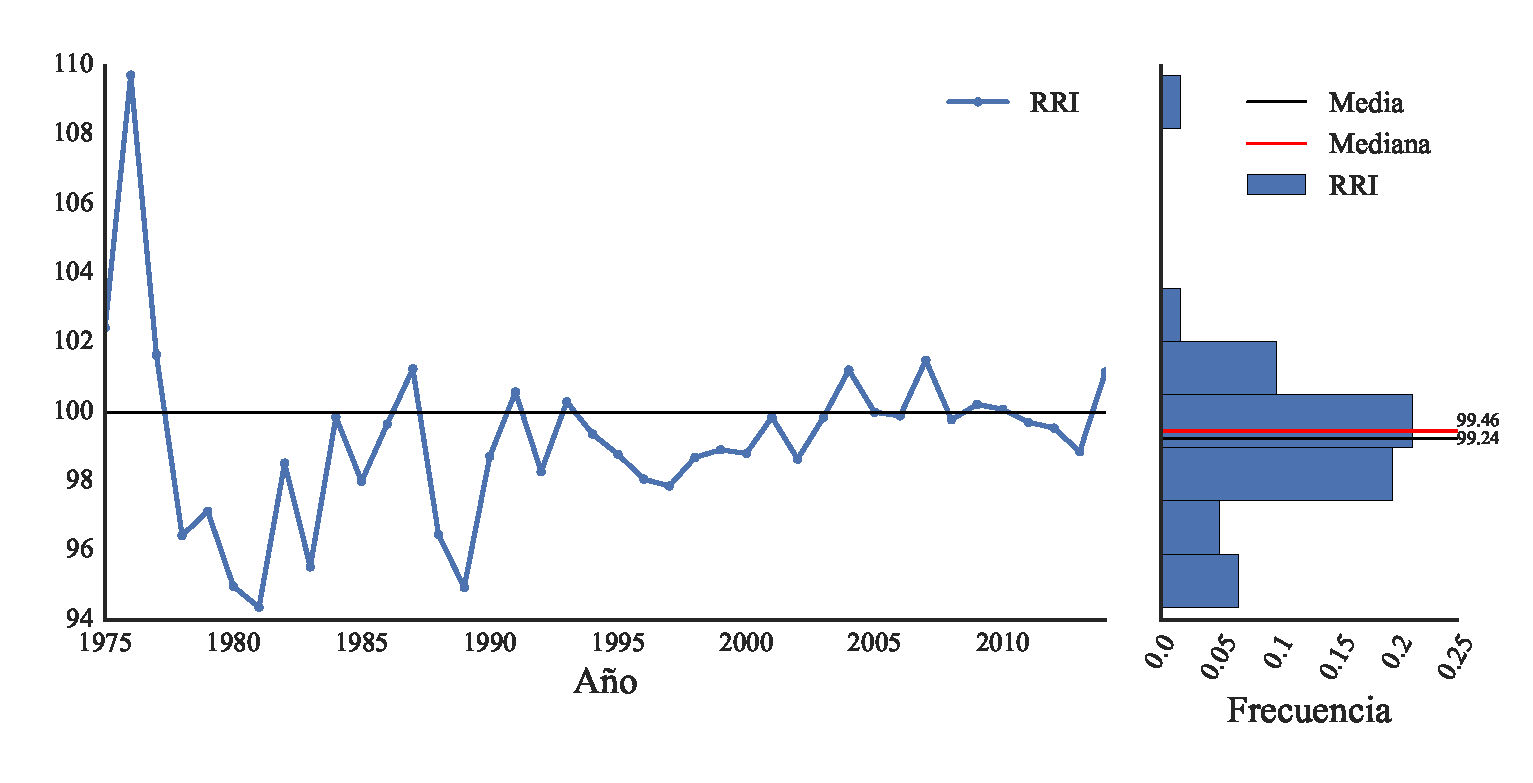
\includegraphics[width=300px]{rri_0}
    \caption*{\textit{Fuente}: Elaboración propia con datos de \textit{World Bank API (WDI)}}
    \label{rri}
\end{figure}

Cómo puede verse en al Figura \ref{rri}, la evolución de la relación real de intercambio de Chipre, gira en torno a un valor por debajo del 100\%, aproximadamente 99.46\% es el porcentaje medio y 99.24\% es el valor de la mediana, como puede constatarse en el histograma de la derecha, mas del 50\% de las observaciones la RRI de chipre se hallan con valores inferiores al 99.24\%, esto estrictamente indica que Chipre pierde bienestar con el comercio internacional, dado que el valor de lo que importa es superior a lo que exporta, lo que implica que para una mismca cantidad de exportaciones cada vez puede importar menos. En el periodo analizado sin duda Chipre ha perdido bienestar con el comercio internacional con más frecuencia que el que ha ganado.


\chapter{Evolución Del Comercio}
\label{cap2EvoComer}

Tanto las importaciones cómo las exportaciones se han visto afectadas nominalmente en 2008 por la crisis económica, afectando al comercio internacional de Chipre como muestra la tabla 2. En los últimos 10 años, el crecimiento de ambas variables ha girado en torno al 2\% siendo las exportaciones ligeramente superior a las importaciones haciendo que el crecimiento del saldo exterior sea positivo pero muy discreto, de una magnitud cercana al 0,2\%. Es interesante que ver que sólo dos años (el 20\% de los datos ) el crecimiento de las exportaciones presentó valores negativos y en el caso de las importaciones tres datos (30\%).

% Please add the following required packages to your document preamble:
% \usepackage{booktabs}
\begin{table}[]
    \centering
    \caption{Evolución Comercio}
    \label{tab_evocomer}
    \resizebox{\textwidth}{!}{%
        \begin{tabular}{@{}llllllllllll@{}}
        \toprule
        AÑO                                                 & 2004     & 2005      & 2006      & 2007      & 2008      & 2009      & 2010      & 2011      & 2012      & 2013      & 2014      \\ \midrule
        Exportaciones de bienes y servicios (corriente LCU) & 7,88E+09 & 8,25E+09  & 8,55E+09  & 9,33E+09  & 9,42E+09  & 8,72E+09  & 9,10E+09  & 9,65E+09  & 9,65E+09  & 9,21E+09  & 9,70E+09  \\
        Importaciones de bienes y servicios (corriente LCU) & 7,90E+09 & 8,33E+09  & 9,02E+09  & 1,02E+10  & 1,14E+10  & 9,55E+09  & 1,02E+10  & 1,03E+10  & 1,00E+10  & 8,76E+09  & 9,22E+09  \\
        Crecimiento nominal de las exportaciones            & 6,24     & 4,72      & 3,57      & 9,08      & 0,97      & -7,39     & 4,29      & 6,13      & 0,00      & -4,59     & 5,37      \\
        Crecimiento nominal de las importaciones            & 9,35     & 5,49      & 8,23      & 12,64     & 12,61     & -16,52    & 6,36      & 1,59      & -2,82     & -12,65    & 5,26      \\
        Exportaciones de bienes y servicios (constante LCU) & 8,09E+09 & 8,25E+09  & 8,36E+09  & 8,80E+09  & 8,65E+09  & 8,02E+09  & 8,23E+09  & 8,58E+09  & 8,43E+09  & 8,01E+09  & 8,47E+09  \\
        Importaciones de bienes y servicios (constante LCU) & 8,21E+09 & 8,33E+09  & 8,81E+09  & 9,73E+09  & 1,05E+10  & 8,80E+09  & 9,20E+09  & 9,14E+09  & 8,72E+09  & 7,54E+09  & 8,14E+09  \\
        Crecimiento real de las exportaciones               & 2,49     & 2,05      & 1,27      & 5,28      & -1,72     & -7,28     & 2,63      & 4,21      & -1,66     & -4,99     & 5,72      \\
        Crecimiento real de las importaciones               & 6,95     & 1,57      & 5,70      & 10,46     & 7,74      & -16,05    & 4,52      & -0,62     & -4,60     & -13,61    & 8,07      \\
        Saldo comercial (Moneda local)                      & 1,89E+08 & -7,90E+07 & -6,60E+08 & -1,36E+09 & -2,79E+09 & -1,53E+09 & -1,93E+09 & -1,74E+09 & -1,59E+09 & -7,45E+08 & -7,48E+08 \\
        Saldo comercial (\% PIB)                            & -0,13    & -0,54     & -2,97     & -4,81     & -10,78    & -4,50     & -5,57     & -3,42     & -1,93     & 2,48      & 2,76      \\
        Tasa de cobertura (\%)                              & 99,78    & 99,05     & 94,79     & 91,80     & 82,32     & 91,32     & 89,54     & 93,55     & 96,26     & 105,14    & 105,25    \\
        Tasa de apertura (\%)                               & 114,94   & 112,92    & 110,94    & 112,45    & 111,13    & 99,18     & 101,00    & 102,49    & 101,39    & 99,18     & 108,10    \\
        Penetración de importaciones (\%)                   & 57,46    & 56,42     & 55,31     & 55,94     & 55,02     & 49,61     & 50,47     & 51,20     & 50,68     & 49,58     & 54,17     \\
        Propensión exportadora (\%)                         & 57,41    & 56,19     & 53,99     & 53,82     & 50,18     & 47,34     & 47,71     & 49,54     & 49,73     & 50,83     & 55,43     \\
        PIB (corriente LCU)                                 & 1,37E+10 & 1,47E+10  & 1,58E+10  & 1,73E+10  & 1,88E+10  & 1,84E+10  & 1,91E+10  & 1,95E+10  & 1,94E+10  & 1,81E+10  & 1,75E+10  \\
        PIB (constante LCU)                                 & 1,41E+10 & 1,47E+10  & 1,54E+10  & 1,61E+10  & 1,67E+10  & 1,64E+10  & 1,66E+10  & 1,67E+10  & 1,62E+10  & 1,53E+10  & 1,49E+10  \\ \bottomrule
        \end{tabular}}
    \caption*{\textit{Fuente}: Elaboración propia con datos de World Bank API.}

\end{table}

% Please add the following required packages to your document preamble:
% \usepackage{booktabs}
\begin{table}[]
    \centering
    \caption{Determinantes de las exportaciones}
    \label{2DeterX}
    \resizebox{\textwidth}{!}{%
        \begin{tabular}{@{}lrrrrrrrrrrrr@{}}
        \toprule
        AÑO                                                             & 2003     & 2004     & 2005     & 2006     & 2007     & 2008     & 2009     & 2010     & 2011     & 2012     & 2013     & 2014     \\ \midrule
        CUADRO DETERMINANTES DE LAS EXPORTACIONES                       &          &          &          &          &          &          &          &          &          &          &          &          \\
        DATOS ORIGINALES                                                &          &          &          &          &          &          &          &          &          &          &          &          \\
        Exportaciones de bienes y servicios Chipre  (constante LCU)     & 7,89E+09 & 8,09E+09 & 8,25E+09 & 8,36E+09 & 8,80E+09 & 8,65E+09 & 8,02E+09 & 8,23E+09 & 8,58E+09 & 8,43E+09 & 8,01E+09 & 8,47E+09 \\
        PIB Grecia (constante LCU)                                      & 2,17E+11 & 2,28E+11 & 2,30E+11 & 2,43E+11 & 2,51E+11 & 2,50E+11 & 2,39E+11 & 2,26E+11 & 2,05E+11 & 1,90E+11 & 1,84E+11 & 1,86E+11 \\
        Tipo de cambio oficial Chipre (LCU por US\$, media del periodo) & 0,52     & 0,47     & 0,46     & 0,46     & 0,43     & 1,00     & 1,00     & 1,00     & 1,00     & 1,00     & 1,00     & 1,00     \\
        Tipo de cambio oficial Grecia (LCU por US\$, media del periodo) & 0,89     & 0,81     & 0,80     & 0,80     & 0,73     & 0,68     & 0,72     & 0,76     & 0,72     & 0,78     & 0,75     & 0,75     \\
        IPC Chipre (2010 = 100)                                         & 80,08    & 82,40    & 85,32    & 88,05    & 90,60    & 94,36    & 95,50    & 100,00   & 103,33   & 104,88   & 103,92   & 102,55   \\
        IPC Grecia (2010 = 100)                                         & 84,46    & 86,39    & 88,60    & 90,81    & 92,97    & 97,31    & 97,67    & 100,00   & 103,29   & 105,76   & 105,33   & 103,91   \\
        DATOS RELATIVOS                                                 &          &          &          &          &          &          &          &          &          &          &          &          \\
        Tipo de cambio Chipre/Grecia                                    & 0,58     & 0,58     & 0,58     & 0,58     & 0,58     & 1,46     & 1,39     & 1,32     & 1,39     & 1,28     & 1,33     & 1,33     \\
        Índice de precios Chipre/Grecia                                 & 0,95     & 0,95     & 0,96     & 0,97     & 0,97     & 0,97     & 0,98     & 1,00     & 1,00     & 0,99     & 0,99     & 0,99     \\
                                                                        &          &          &          &          &          &          &          &          &          &          &          &          \\
        TASAS DE CRECIMIENTO                                            &          &          &          &          &          &          &          &          &          &          &          &          \\
        ∆ Real X Chirpe                                                 &          & 2,49     & 2,05     & 1,27     & 5,28     & -1,72    & -7,28    & 2,63     & 4,21     & -1,66    & -4,99    & 5,72     \\
        ∆ Real PIB Chipre                                               &          & 5,06     & 0,60     & 5,65     & 3,27     & -0,34    & -4,30    & -5,48    & -9,13    & -7,30    & -3,20    & 0,65     \\
        ∆ Tipo de cambio Chipre / Grecia                                &          & -0,37    & -0,81    & -0,24    & 1,31     & 151,16   & -5,16    & -4,66    & 4,96     & -7,57    & 3,34     & -0,08    \\
        ∆ IPR Chipre / Grecia                                           &          & 0,60     & 0,96     & 0,68     & 0,51     & -0,49    & 0,83     & 2,28     & 0,04     & -0,87    & -0,52    & 0,04     \\ \bottomrule
        \end{tabular}}
    \caption*{\textit{Fuente}: Elaboración propia con datos de World Bank API.}
\end{table}

Ambos gráficos presentan un patrón bien conocido en economía, en forma de “W”, se pueden distinguir, para ambos gráficos, que desde 2004 hasta finales de 2007 los crecimientos nominales y reales de las importaciones y exportaciones son positivas, aunque no se aprecia una tendencia clara, pero si que en 2007 se alcanza un máximo en ambas variables.

Con la llegada de la crisis se alcanzan tasas de crecimiento mínimas en 2009 observándose luego un repunte en 2010 y otra caída en 2013 y un último pico final.
Notar que el crecimiento real tanto de las importaciones como de las exportaciones está siempre por debajo del nominal, lo que indica que hay inflación, resaltar que en el último periodo en donde el crecimiento real supera ligeramente al nominal, indicando deflación en dichos bienes.

La tabla \ref{2DeterX}, nos informa del saldo comercial, que ha sido deficitario hasta los último dos años, que presenta, valores positivos tanto en porcentaje de PIB cómo en valor absoluto. En sincronía  redundancia con lo anterior, la tasa de cobertura es menor que 100 salvo en los dos últimos periodos. La tasa de apertura de Chipre, se ha mantenido en niveles similares durante el periodo, si bien es cierto que ha ido cayendo ligeramente y esto podría indicar que aumenta su mercado interno.

La penetración de las importaciones es una medida de dependencia de una economía, mide el porcentaje de demanda interna satisfecha vía importaciones, vemos que Chipre se ha mantenido en valores muy estables al rededor del 50%.

La propensión exportadora que mide el porcentaje de producción que se dirige a la exportación es muy similar al anterior indicador y también se mantiene en niveles por encima del 50\%

\begin{figure}[ht]
    \caption{Evolución de las Importaciones (por uno) y su frecuencia.}
    \centering
    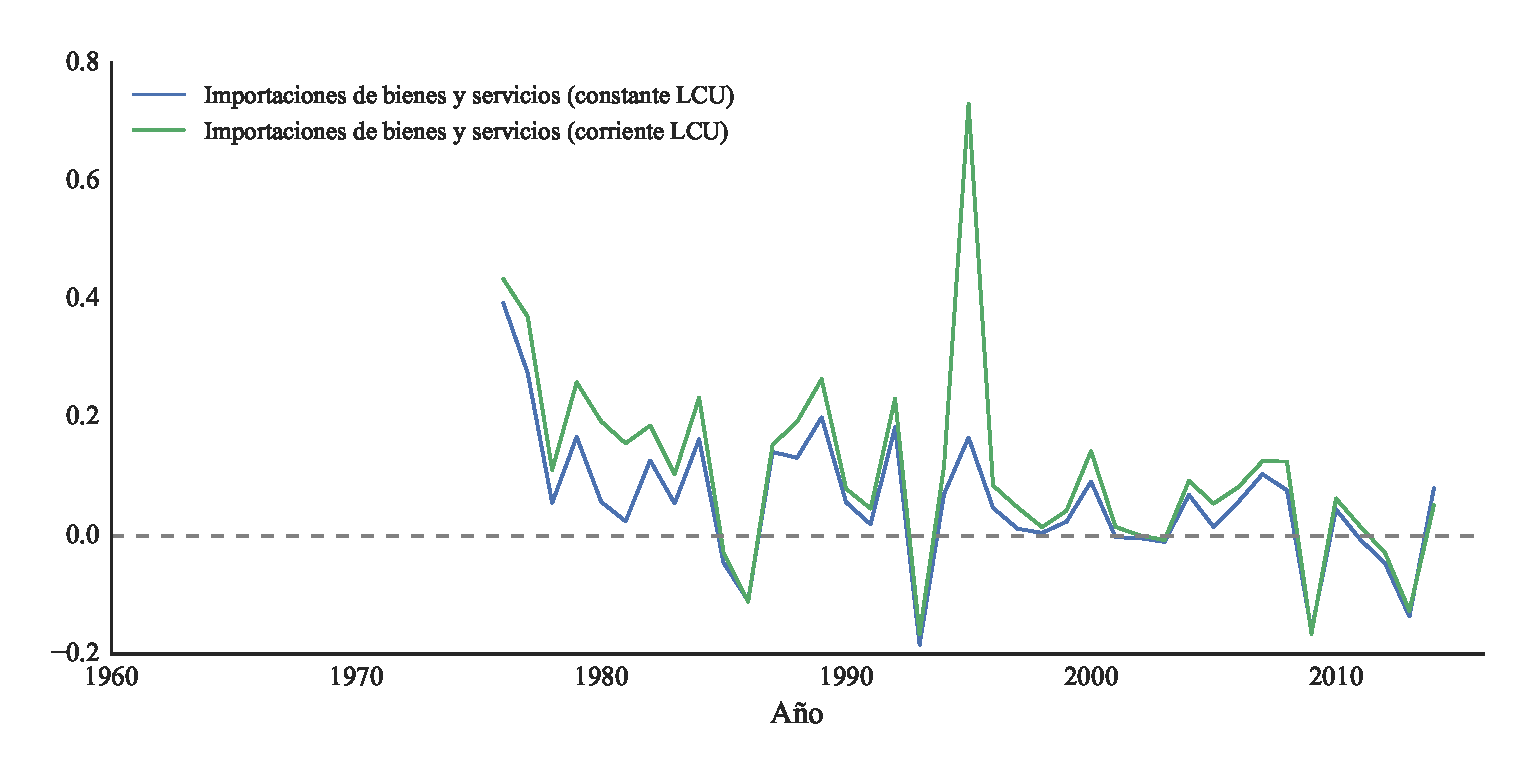
\includegraphics[width=300px]{ev_m}
    \label{ev_m}
\end{figure}

\begin{figure}[ht]
    \caption{Evolución de las Exportaciones (por uno) y su frecuencia.}
    \centering
    \includegraphics[width=300px]{ev_x}
    \label{ev_x}

\end{figure}
\begin{figure}[ht]
    \caption{Evolución de las Exportaciones (por uno) y su frecuencia.}
    \centering
    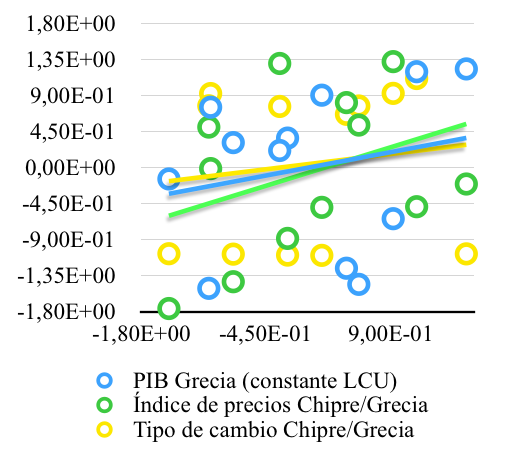
\includegraphics[width=300px]{disp_x.png}
    \label{disp_x}
\end{figure}

\begin{figure}[ht]
    \caption{Evolución de las Exportaciones (por uno) y su frecuencia.}
    \centering
    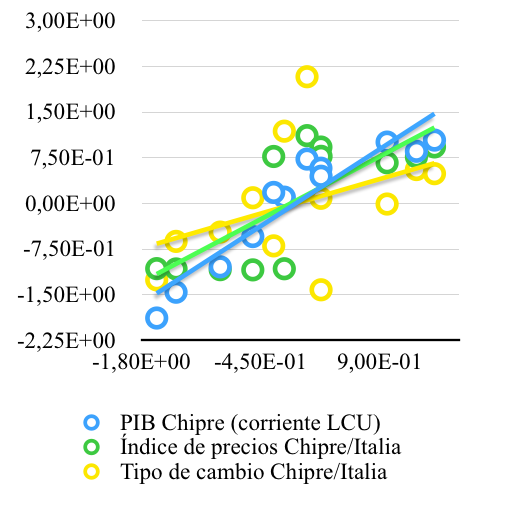
\includegraphics[width=300px]{disp_m.png}
    \label{disp_m}
\end{figure}

En la figura 6 no se aprecia ninguna conclusión evidente, parte de ello es debido a la presencia de un outlier en 2008 en la variable ∆TDC Chipre/Grecia que desvirtúa la escala.
Para intentar ver alguna relación, he normalizado de la Tabla 3 las variables presentes en la Figura 6. La normalización consiste en restar la media y dividir por la desviación típica la variables, de forma que éstas sean comparables entre si.
En la figura 7 se representa la dispersión de las variables frente a las exportaciones, la linea de regresión lineal nos proporciona una buena aproximación del efecto de cada variable sobre las exportaciones.

El PIB de Grecia, afecta positivamente, justo como era de esperar teóricamente, el IPR tiene un efecto positivo mientras que en teoría el efecto de los precios es negativo, y por último el TDC afecta positivamente tal y cómo predice la teoría.

\chapter{Distribución Geográfica De M y X}
\label{cap3}

En este apartado se analizan cuales son los principales socios comerciales de  Chipre, tanto proveedores cómo clientes, y se identifican las posibles causas explicativas para que sean esos países y no otros.
En primer lugar, se presentan los pesos de las exportaciones e importaciones por países con el fin de identificar los principales socios de Chipre. En segundo lugar, se obtienen y muestran los principales países a los que Chipre exporta, con lo que se identifica los principales clientes de Chipre. De esta forma tenemos caracterizados los clientes y proveedores.
En la base de datos PC-TAS, obtenemos los principales socios comerciales, exportando los datos de allí, y ordenando los pesos tenemos dos tablas, que se resumen en las siguientes figuras 10 y sucesivas:

\begin{figure}[ht]
    \centering
    \caption{Peso de las importaciones para los principales socios comerciales}
    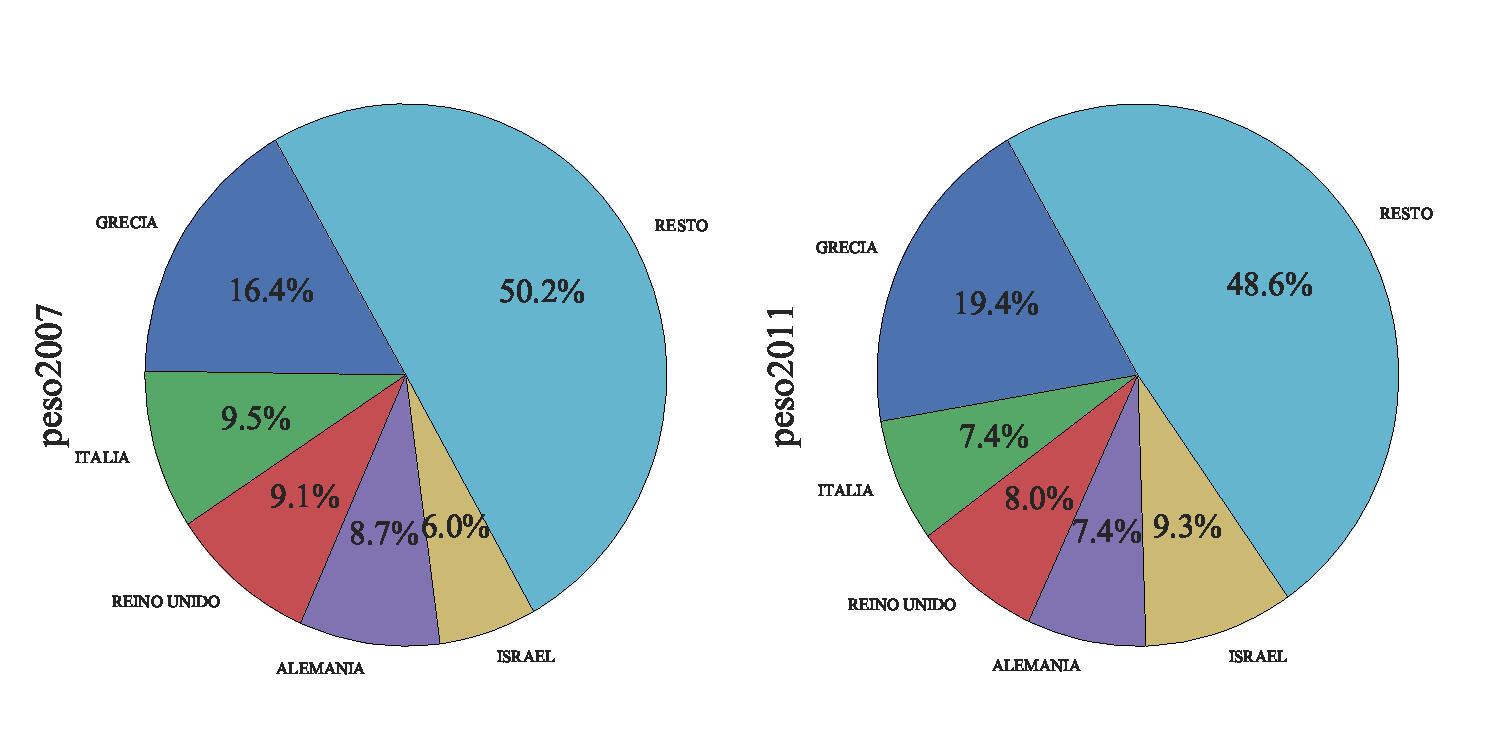
\includegraphics[width=350px]{pie_mgeo.pdf}
    \caption*{\textit{Fuente}: Elaboración propia con datos de \textit{PC-TAS}}
    \label{pie_mgeo}
\end{figure}

\begin{figure}[ht]
    \centering
    \caption{Peso de las importaciones de los principales socios comerciales}
    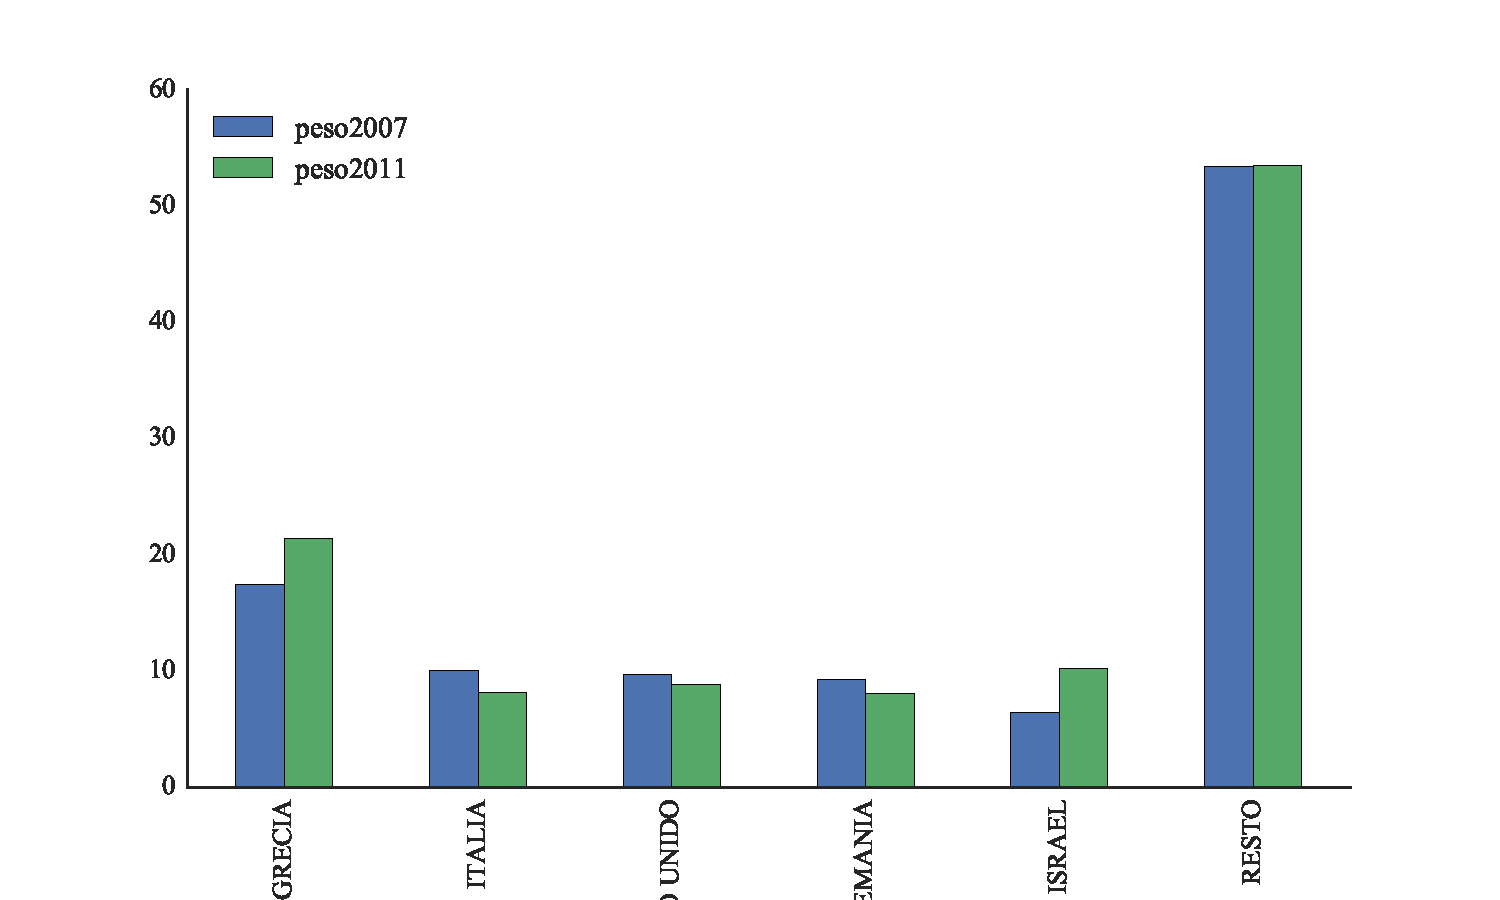
\includegraphics[width=350px]{bar_mgeo.pdf}
    \caption*{\textit{Fuente}: Elaboración propia con datos de \textit{PC-TAS}}
    \label{bar_mgeo}
\end{figure}


Las exportaciones de Chipre (tabla 5) tienen como principales destinos, Grecia, Para Buques, Reino Unido, Alemania y Rumanía, que juntas tiene un peso de 58,69\% en 2007 y 56,79\% en 2011. Cómo puede verse en la tabla 6, las exportaciones de 2007 hacia Grecia y Para Buques aumentaron en 2011, mientras que el resto disminuyeron.
Los principales orígenes de las importaciones de Chipre son países de la propia unión europea como muestra la Figura REF, pero destaca sobre el resto las importaciones procedentes de Grecia con casi el doble de peso sobre el esto, diferencia que se ha mantenido desde 2007 hasta 2011.


\begin{figure}[ht]
    \centering
    \caption{Peso de las exportaciones de los principales socios comerciales}
    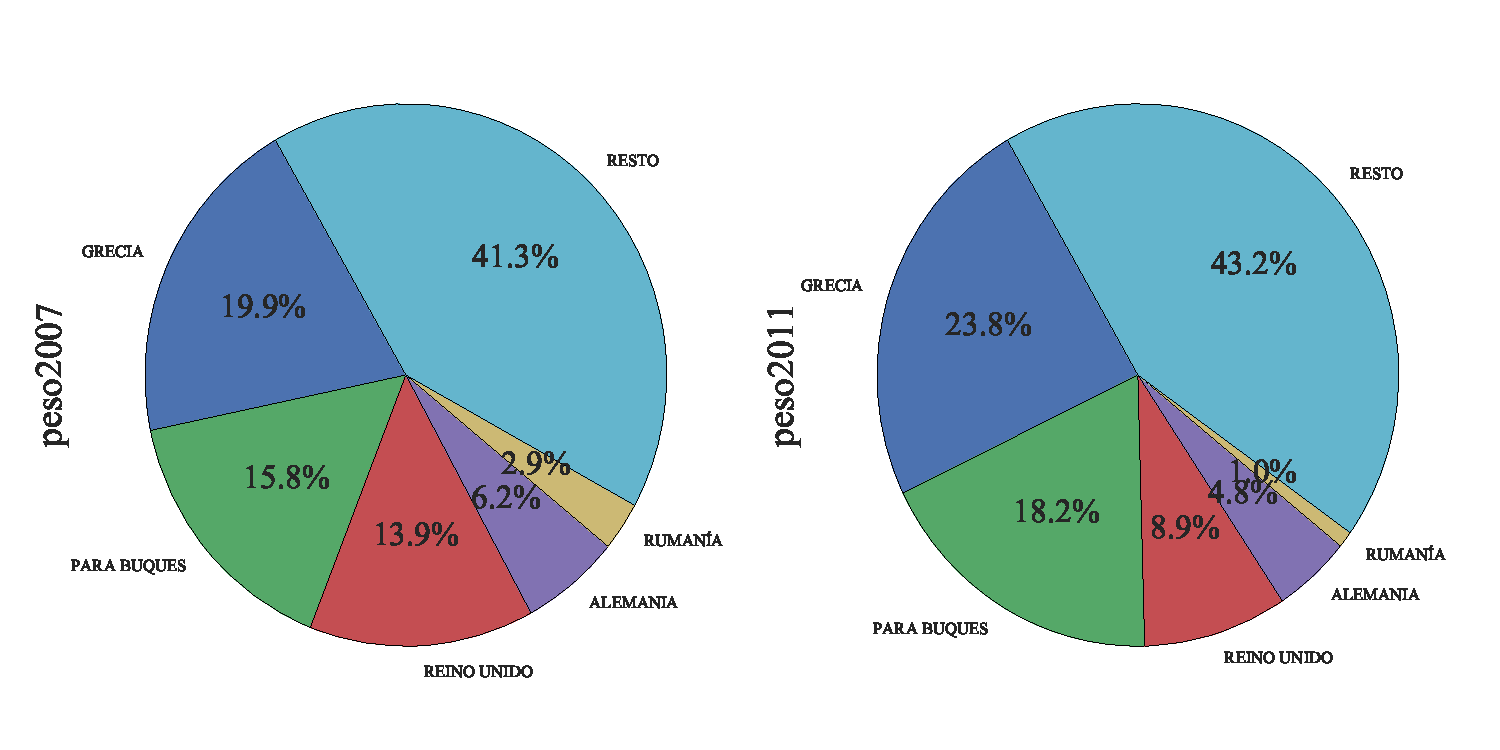
\includegraphics[width=350px]{pie_xgeo.pdf}
    \caption*{\textit{Fuente}: Elaboración propia con datos de \textit{PC-TAS}}
    \label{pie_xgeo}
\end{figure}

\begin{figure}[tbh]
    \centering
    \caption{Peso de las exportaciones de los principales socios comerciales}
    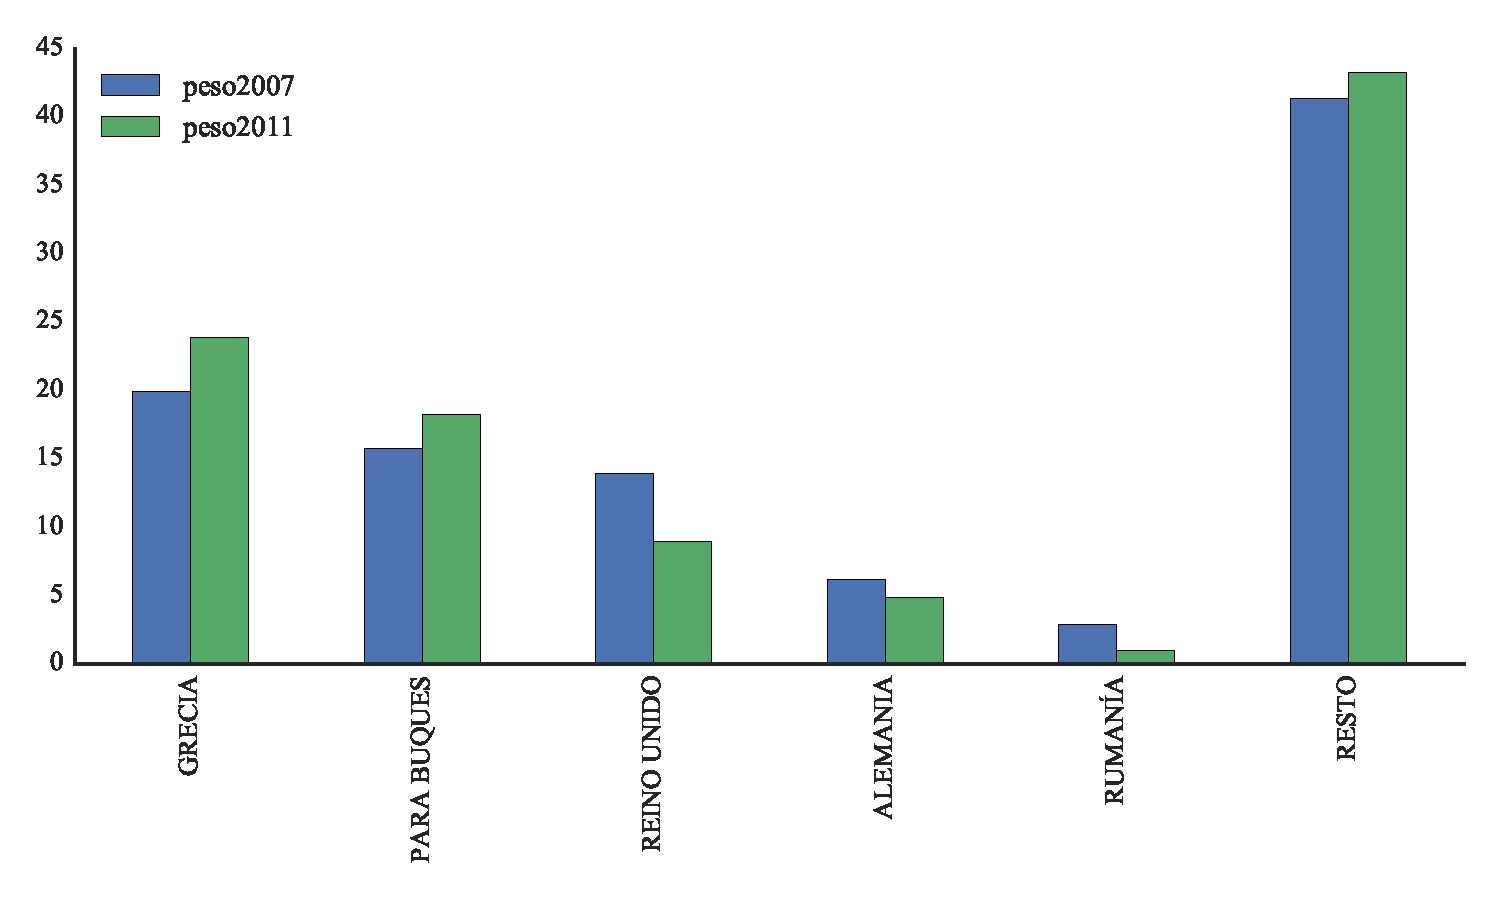
\includegraphics[width=350px]{bar_xgeo.pdf}
    \caption*{\textit{Fuente}: Elaboración propia con datos de \textit{PC-TAS}}
    \label{bar_xgeo}
\end{figure}

Sobre las importaciones los principales proveedores de Chipre son Grecia, Italia, Reino Unido, Alemania e Israel. Como puede apreciarse en la tabla 5 los principales clientes son Grecia, Para Naves (casa especial debido a las bases militares ubicadas en Chipre), Reino Unido, Alemania, Líbano, Italia y Emiratos Arabes.

Los destinos concuerdan con la historia Chipriota, fue una colonia y de Reino Unido, y formó parte de Grecia, esta dependencia del pasado ha hecho que se mantenga hasta hoy en día nexos comerciales fuertes. Estas relaciones se pueden explicar viendo el pasado geopolítico de Chipre, que pasó a estar a menos de UK, luego Grecia.

\subsubsection{El modelo de Gravedad}

Según el modelo de gravedad en su forma más general, definida de la siguiente manera:

\begin{equation}
T_{ij} = A \cdot Y_i^a \cdot \frac{Y_j^b}{D_{ij}^c}
\end{equation}

dónde, $T_i_j$ es el valor del comercio entre el país _i_ y el país _j_, $Y_i^a$ es el PIB del país _i_, $Y_j^b$ es el PIB del país j y $D_i_j$ es la distancia entre los dos países

La pregunta que cabe hacerse es si el comercio entre Chipre y estos países siguen el comportamiento previsto por el modelo de gravedad, y para eso hay que analizar la distancia entre los países, el PIB. A priori, sin datos, Reino Unido tiene una distancia menor y un PIB mayor que Grecia, sin embargo, el peso de las exportaciones es menor que el de Grecia, esto a grandes rasgos sugiere que no se cumple el modelo de Gravedad, para un análisis riguroso necesitamos, los datos y hacer un análisis econométrico.

\chapter{Competitividad Precio O Coste}
\label{cap4}

% Please add the following required packages to your document preamble:
% \usepackage{booktabs}
\begin{table}[h]
    \centering
    \caption{Resúmen}
    \label{my-label}
    \resizebox{\textwidth}{!}{%
    \begin{tabular}{@{}lrrrrrrrrrrr@{}}
    \toprule
    DATOS ORIGINALES                            &        &        &        &        &        &        &        &        &        &        &        \\
                                                & 2005   & 2006   & 2007   & 2008   & 2009   & 2010   & 2011   & 2012   & 2013   & 2014   & 2015   \\ \midrule
    Tipo de cambio Chipre                       & 0,46   & 0,46   & 0,43   & 0,68   & 0,72   & 0,76   & 0,72   & 0,78   & 0,75   & 0,75   & 0,90   \\
    Tipo de cambio Italia                       & 0,80   & 0,80   & 0,73   & 0,68   & 0,72   & 0,76   & 0,72   & 0,78   & 0,75   & 0,75   & 0,90   \\
    Tipo de cambio Grecia                       & 0,80   & 0,80   & 0,73   & 0,68   & 0,72   & 0,76   & 0,72   & 0,78   & 0,75   & 0,75   & 0,90   \\
    Indice de precios Chipre                    & 88,60  & 90,81  & 92,97  & 97,31  & 97,67  & 100,00 & 103,29 & 105,76 & 105,33 & 103,91 & 101,73 \\
    Indice de precios Italia                    & 90,98  & 92,87  & 94,56  & 97,75  & 98,48  & 100,00 & 102,74 & 105,87 & 107,16 & 107,42 & 107,46 \\
    Indice de Precios Grecia                    & 85,32  & 88,05  & 90,60  & 94,36  & 95,50  & 100,00 & 103,33 & 104,88 & 103,92 & 102,55 & 100,77 \\
                                                &        &        &        &        &        &        &        &        &        &        &        \\
    INDICE DE TIPO DE CAMBIO EFECTIVO REAL      &        &        &        &        &        &        &        &        &        &        &        \\
    DATOS REALTIVOS                             &        &        &        &        &        &        &        &        &        &        &        \\
                                                & 2005   & 2006   & 2007   & 2008   & 2009   & 2010   & 2011   & 2012   & 2013   & 2014   & 2015   \\ \midrule
    Tipo de cambio Chipre/Italia                & 57,71  & 57,57  & 58,32  & 100,00 & 100,00 & 100,00 & 100,00 & 100,00 & 100,00 & 100,00 & 100,00 \\
    Tipo de cambio Chipre/Grecia                & 57,71  & 57,57  & 58,32  & 100,00 & 100,00 & 100,00 & 100,00 & 100,00 & 100,00 & 100,00 & 100,00 \\
    Precios relativos Chipre/Italia             & 97,38  & 97,79  & 98,32  & 99,55  & 99,18  & 100,00 & 100,53 & 99,90  & 98,30  & 96,73  & 94,67  \\
    Precios relativos Chipre/Grecia             & 103,85 & 103,14 & 102,62 & 103,13 & 102,28 & 100,00 & 99,96  & 100,84 & 101,37 & 101,32 & 100,95 \\
    Indice de tipo de cambio real Chipre/Italia & 56,20  & 56,30  & 57,34  & 99,55  & 99,18  & 100,00 & 100,53 & 99,90  & 98,30  & 96,73  & 94,67  \\
    Indice de tipo de cambio real Chipre/Grecia & 59,93  & 59,38  & 59,85  & 103,13 & 102,28 & 100,00 & 99,96  & 100,84 & 101,37 & 101,32 & 100,95 \\ \bottomrule
    \end{tabular}
    }
\end{table}

El país seleccionado como principal proveedor se corresponde con el segundo más importante en la relación con el peso de las importaciones de chipre, dado que el de mayor peso coincide con  el paí seleccionado como el principal cliente.

\begin{figure}
    \includegraphics{/path/to/figure}
    \caption{}
    \label{}
    \caption{}
\end{figure}

En el gráfico puede verse la evolución de tres variables, tipo de cambio relativo, precios relativos y el tipo de cambio real relativo. La evolución de los precios relativos se mantiene prácticamente constante durante el período, apreciándose un descenso a partir de 2013 que indica que Chipre está ganando competitividad frente a Italia.

\chapter{Competitividad Estructural}
\label{cap5}

\subsection{Competitividad Estructural Cuota De Mercado}

El país seleccionado como principal proveedor se corresponde con el segundo más importante en la relación con el peso de las importaciones de Chipre, dado que el de mayor peso coincide con  el país seleccionado como el principal cliente.

En el gráfico puede verse la evolución de tres variables, tipo de cambio relativo, precios relativos y el tipo de cambio real relativo. La evolución de los precios relativos se mantiene prácticamente constante durante el período, apreciándose un descenso a partir de 2013 que indica que Chipre está ganando competitividad frente a Italia.
Tabla 8: Competitividad Precio
La tabla 8 recoge datos sobre variables relevantes en la competitividad precio/coste. Destacar que dado que Chipre entro en la UE en 2008 su tipo de cambio paso a unificarse con el resto de miembros y por tanto los datos se han rellenado bajo ese criterio, es decir, usando el tipo de cambio de la UE-28.
Ese hecho queda reflejado en la figura 16 y 17 en el esfuerzo de Chipre en 2008 al ajustarse a los tipos de cambio nominal y real.

La figura 18 muestra la evolución del tipo de cambio efectivo real, muestra una tendencia creciente que se corresponde con una depreciación real, como consecuencia, se abaratan las exportaciones, se encarecen las importaciones y lo que se traduce en una perdida de competitividad.
Este efecto se acucia en 2008 con la entrada de Chipre en la UE, claramente apreciado en las tres figuras 16, 17 y 18, con un salto de nivel en los tipos de cambio (permaneciendo constantes los indices de precios relativos).

Con los datos de 2011 obtenidos de la base de datos PC-TAS, se han calculado las cuotas de mercado (CM) de cada sector i, definida ésta como: el cociente entre las importaciones (exportaciones) de Chipre y la UE:

$$CM = \frac{X_{chipre_i}}{X_{ue_i}}100$$

$$CM = \frac{M_{chipre_i}}{M_{ue_i}} 100$$

Se han seleccionado las cuotas que alcanzan el 25\% más importantes, para lo que se ordenan las cuotas de mayor a menor para normalizar los pesos según la suma total de los pesos con esto podemos calcular la suma acumulada, lo cual nos permite seleccionar el cuantil deseado cuando dicha suma alcanza el 25\%.

Con los sectores más importantes seleccionados, analizamos la competitividad estructural:

Los sectores en los que Chipre tiene cierta fortaleza interior relativa son los que figuran en la tabla 9, como característica todos ellos presentan una cuota inferior al 1\% en la UE. Por tanto son sectores en los que Chipre tiene cierta ventaja (si estuviéramos en competencia perfecta y mercados sin distorsiones). Son sectores en los que por algún motivo (innovación, marketing, etc) Chipre es mas competitiva relativamente que el resto de sectores.



\begin{figure}
    \includegraphics{/path/to/figure}
    \caption{}
    \label{}
    \caption*{}
\end{figure}

\chapter{Especialización comercial}
\label{cap6}

En este apartado se analiza el comercio interindustrial o intersectorial, a partir de a partir de los datos sacados de la base de datos PC-TAS, para realizar el análisis se utilizan tres indicadores y se calculan los sectores más relevantes de la economía de Chipre, con pesos en importaciones y exportaciones superiores al 1% sobre el total.
Las formulas aplicadas se encuentran en el anexo del trabajo, y se corresponden con las nombradas anteriormente.
Los sectores en los que Chipre esta especializada (tiene ventaja comparativa) y los que tiene una mayor dependencia están definidos por tres indicadores saldo comercial relativo (SCR), indice de dependencia (IDEP) y el indice de especialización (IESP). El saldo comercial relativo permite dividir en dos grupos los que tienen valores positivos (ventaja comparativa) y los que presentan valores negativos (desventaja comparativa), los cuales a su vez pueden tener un indice de dependencia (>100 dependiente relativamente de ese sector en relación con el grupo) y de especialización mayor que 100 (especialización de ese sector en relación con el grupo). Dichos sectores pueden representarse en una tabla de contingencia con 4 cuadrantes.

El primero (cuadrante 1) corresponde con SCR > 0 y un IDEP>100 (en este caso no hay sectores que cumplan esta condición), el segundo cuadrante (cuadrante 2) corresponde con SCR>0 y un IESP>100, el cuadrante 3 corresponde SCR<0 y un IDEP>100, y por ultimo el cuarto cuadrante corresponde a un SCR<0 y un IESP>100.
Ver Tabla 6 del anexo

Notar que no hay tabla correspondiente al cuadrante 1, esto se debe a que no tiene sectores que cumplan dichos criterios de selección.


% cuadrante 2

Este cuadrante presenta un saldo comercial relativo lo que indica que tiene un superávit en dicho sector de ese tipo de bienes y por tanto ventaja comparativa, por tanto, es de esperar que si tiene ventaja comparativa tenga un indice de especialización alto, pues puede exportar dichos bienes, vemos que tiene un IESP mayor que cien lo cual coincide con lo esperado.

% cuadrante 3

El cuadrante 3 presenta SCR negativo lo que indica desventaja comparativa, y con un IDEP mayor que cien, indica que efectivamente al tener desventaja se espera que tenga que importar este tipo de bienes mas que la UE.


% cuadrante 4

Chipre tiene deficit de este tipo de bienes indicado por SCR negativo, sin embargo, tiene un IESP mayor que cien, indicando que la participación de dicho sector en la exportación es superior al de la UE, lo cual, sugiere presencia de comercio intraindustrial que se analiza en el siguiente epígrafe.

\begin{figure}[ht]
    \centering
    \caption{Distribución de sectores por SCR vs IDEP, IESP}
    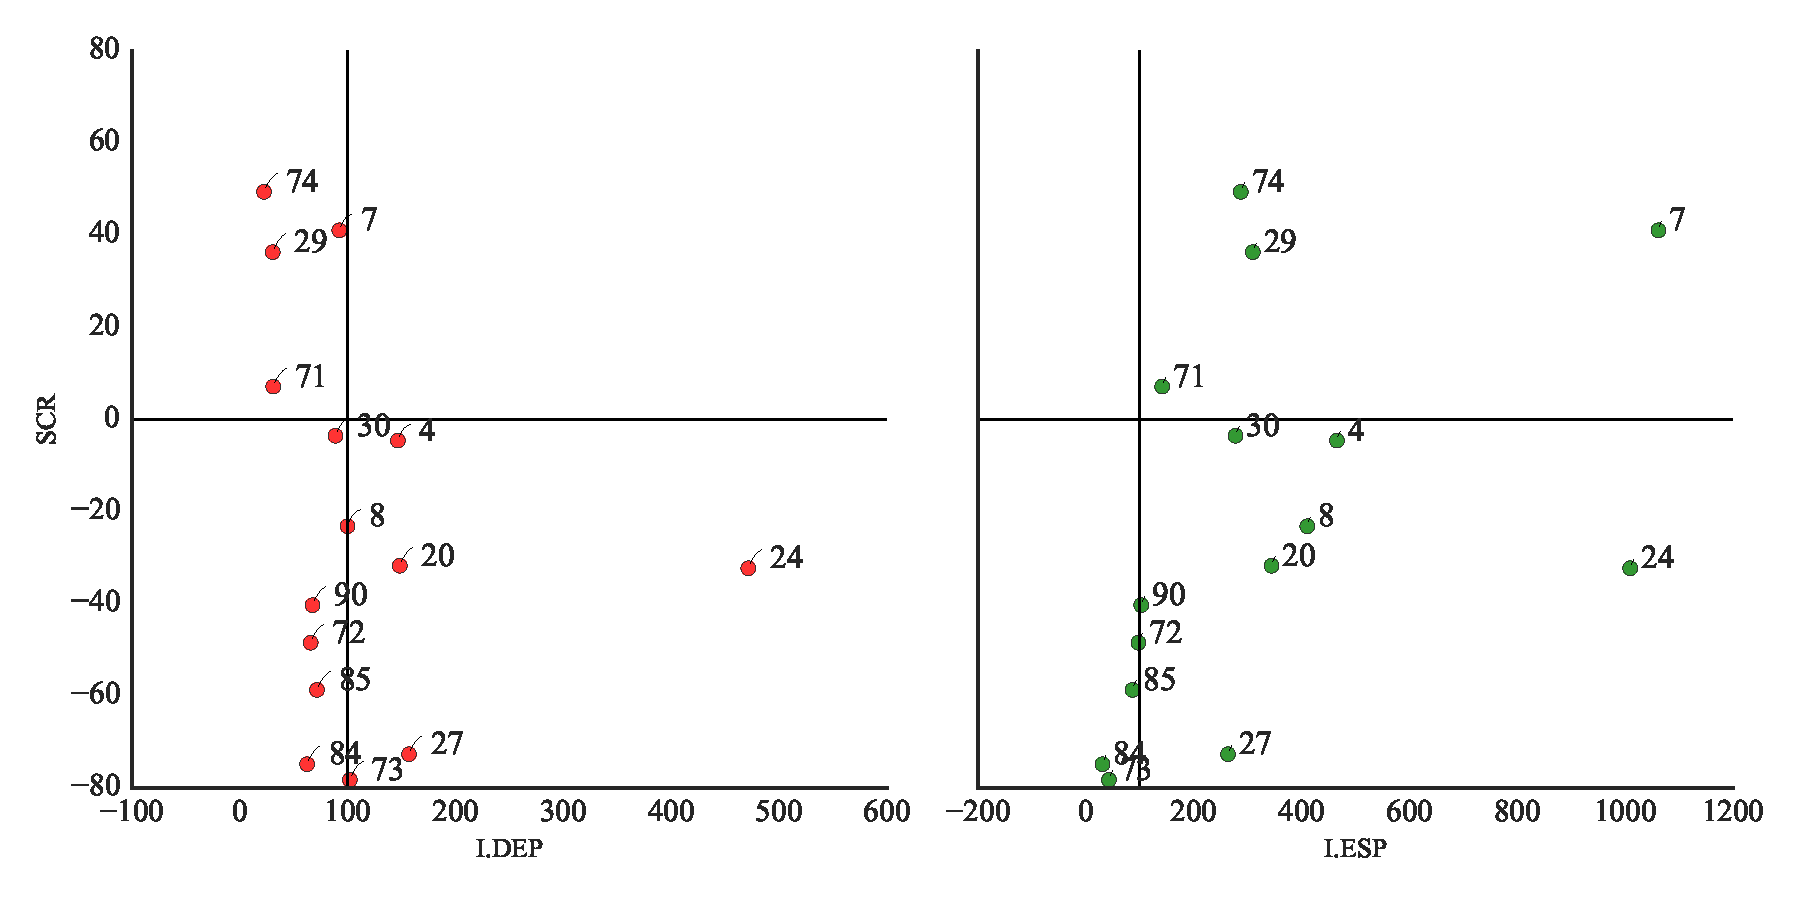
\includegraphics[width=400px]{cuadrantes2.pdf}
    \caption*{\textit{Fuente}: Elaboración propia con datos de \textit{PC-TAS}}
    \label{sec_scr_idep_iesp}
\end{figure}


\chapter{Comercio Intraindustrial}

$$IGL = \frac{X_i + M_i - |X_i - M_i|}{X_i + M_i}$$

ÍNDICE DE GRUBEL Y LLOYD
% ftp://ftp.fundacionsepi.es/pie/dt8902.pdf
Dado el índice de Grubel y Lloyd, vemos que el sector #5 tiene un igl = 1 lo que implica que en ese sector todo el comercio es intraindustrial y no hay comercio interindustrial. Este índices nos proporciona una aproximación al nivel de integración comercial.

% https://docs.google.com/document/d/1EEFpTfqfZyp2Pw_EfPlD7Y8RtGPlCUO55UYHjyqALfA/edit#


Este capítulo se centra en el análisis del comercio intraindustrial de Chipre, para lo cual, se analizan un conjunto de indicadores a partir de los datos obtenidos de la BBDD, Pc-Tas sobre importación y exportación de Chipre. Los datos están desagregado por sectores y por destino/origen. Una descripción de los indicadores usados se encuentra en el \ref{anexo}, entre ellos se usarán: el peso de las importaciones, el índice de especialización, el índice de dependencia, saldo comercial relativo y el índice de Grubel y Lloyd ## AÑADIR CITA, cada uno en su contexto.

Para anlizar el comercio, se han seleccionado los sectores mas importantes según el peso sobre el PIB y dentro de ese grupo, se han elegido aquellos sectore que tienen un indice de especialización mayor que ### y un índice de dependecia mayor que ###.

En el epígrafe anterior se analiza el comercio intersectorial, sin embargo, encontramos ciertas irregularidades debidas que los indicadores utilizados no eran los indicados para ese tipo de sectores, ya que sugerían cosas incongruentes especialmente en los cuadrantes 2 y 3, esto se debe a que las causas que explican el comercio no son la ventaja comparativa sino otras como la economía de escala, diferenciación de productos, marca, gusto por la diversidad (propios de economías avanzadas), etc.

Para realizar un análisis correcto del comercio intraindustrial, es decir, cuando se producen flujos simultáneos de importaciones y exportaciones de un mismo sector. En el cuadrante 4 del epígrafe anterior, el sector con mayor ICINTRA (IGL), 96,4\% es el que corresponde con el código 30 a productos farmacéuticos, la figura 20 recoge los indices de comercio intraindustrial para lo sectores mas relevantes (los 6 con mayor peso en las exportaciones) puede verse como el epígrafe 30 correspondiente a productos farmacéuticos es el que mayor indice de comercio intraindustrial.

Si analizamos los datos de forma mas detallada en la base de datos PC-TAS para ajustar el resultado anterior recalculamos el índice agregado de Grubel y Lloyd cuyos resultados se encuentran en la tabla 10 del anexo, ya que es el indice calculado previamente no es consistente ya que presenta problemas de agregación estadística obteniendo como resultado un IAGL igual a 83,21\%, en lugar del 96,4\% que teníamos anteriormente.

% cuadro de contigencia, indicadores

\begin{figure}[ht]
    \centering
    \caption{Indicadores de especialización comercial por cuadrantes para cada sector}
    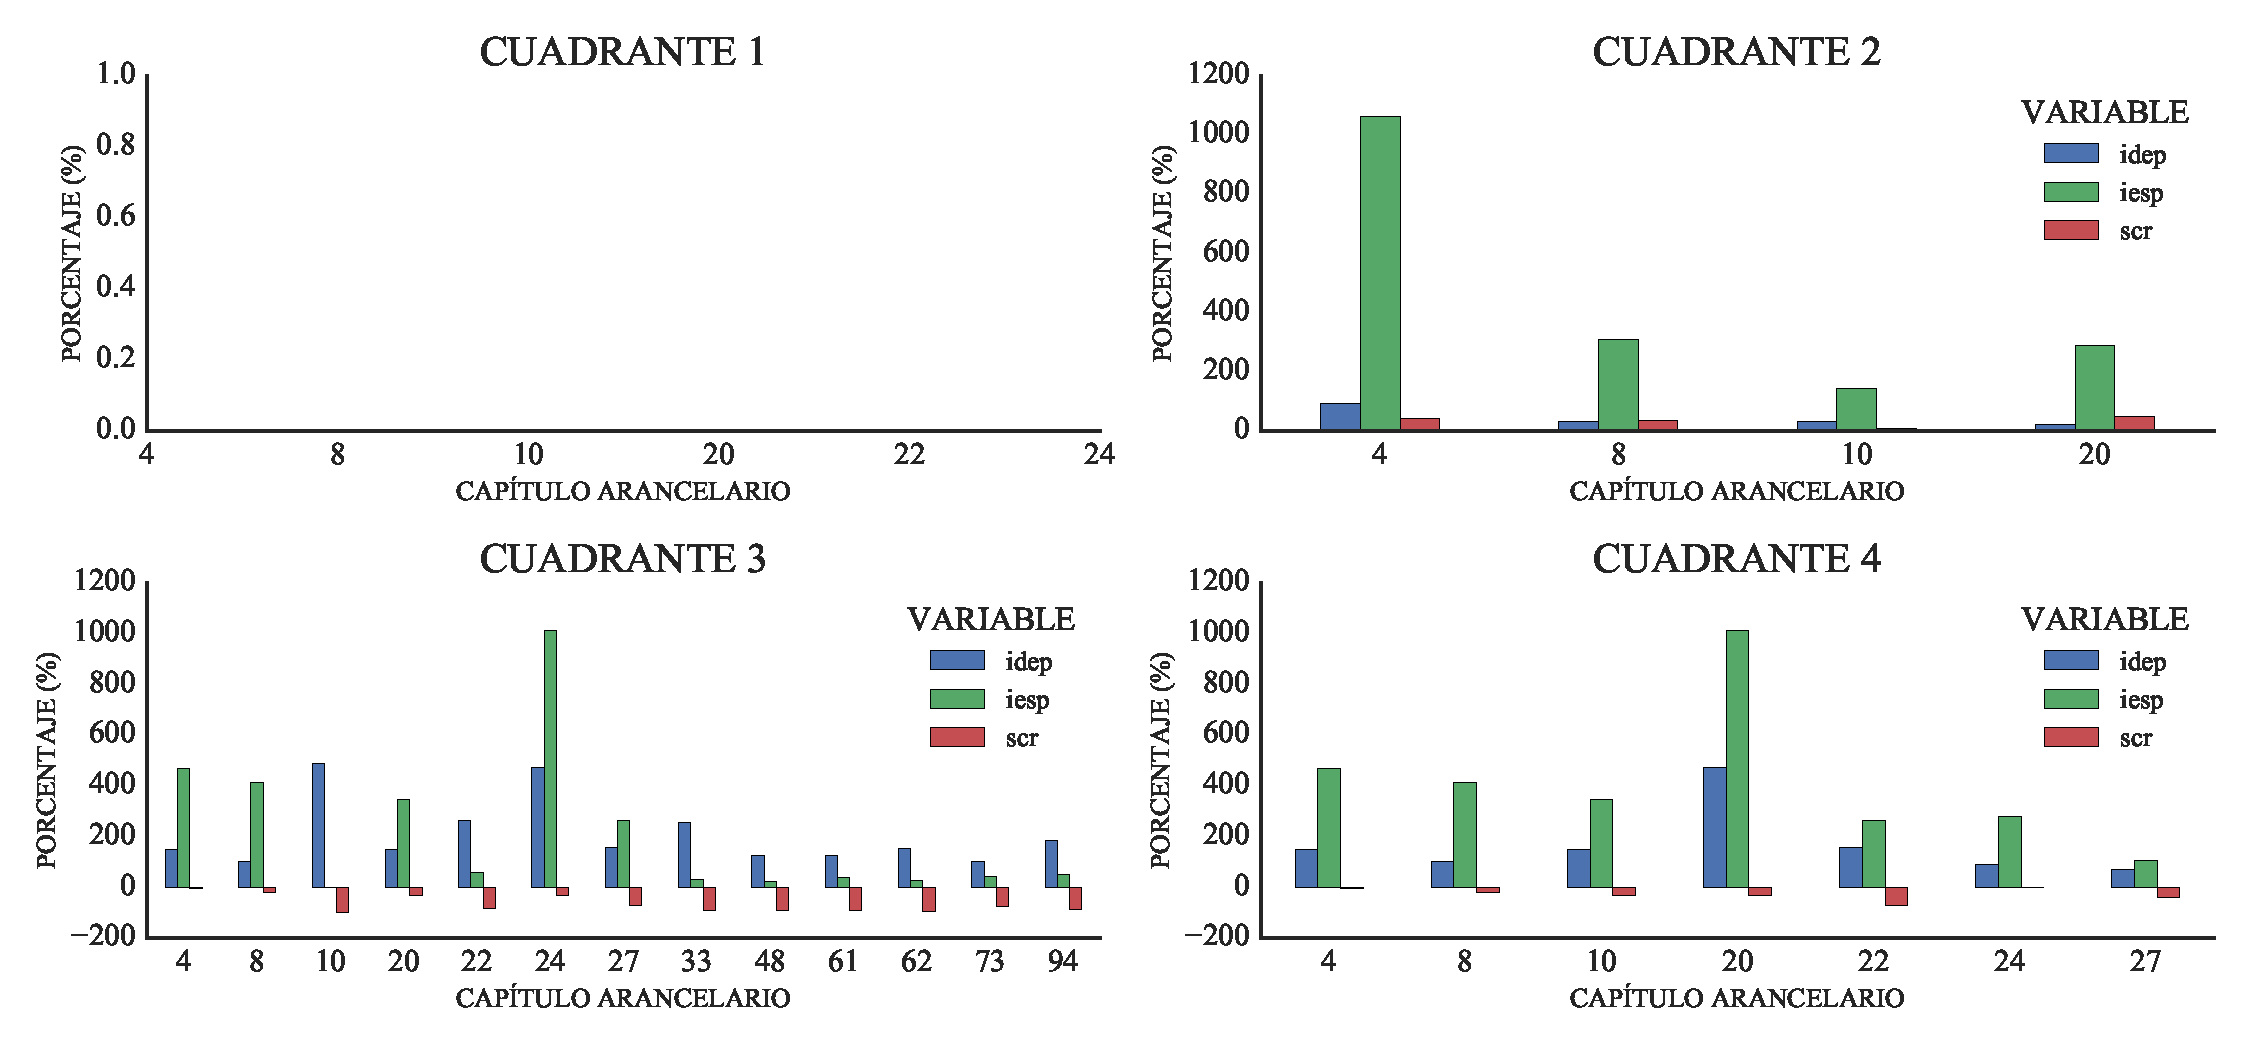
\includegraphics[width=450px]{cuadrantes.pdf}
    \caption*{\textit{Fuente}: Elaboración propia con datos de \textit{PC-TAS}}
    \label{esp_c}
\end{figure}

\begin{table}[ht]
    \centering
    \caption{Descipción de Cuadrantes}
    \label{desc_cuadrantes}
    \begin{tabular}{@{}lcc@{}}
    \toprule
                       & I.DEP \textgreater 100 & I.ESP \textgreater 100 \\ \midrule
    SCR \textgreater 0 & Cuadrante 1      & Cuadrante 2      \\
    SCR \textless 0    & Cuadrante 3  & Cuadrante 4     \\ \bottomrule
    \end{tabular}
\end{table}

% cuadrante 2
\begin{table}[ht]
    \centering
    \caption{Cuadrante 2}
    \label{tab_c2}
    \resizebox{\textwidth}{!}{%
    \begin{tabular}{@{}lllllll@{}}
    \toprule
    & idep                                                                                                          & iesp  & scr      & irx   & irm  & igl  &       \\ \midrule
    Plantas vivas y productos de la floricultura                                                                  & 92,44 & 1.061,90 & 40,98 & 4,40 & 0,41 & 59,02 \\
    Combustibles minerales, aceites minerales y productos de su destilación; materias bituminosas;ceras minerales & 30,67 & 309,79   & 36,25 & 8,74 & 0,92 & 63,75 \\
    Sombreros, demás tocados y sus partes.                                                                        & 31,18 & 141,60   & 7,07  & 2,71 & 0,53 & 92,93 \\
    Manufacturas de piedra, yeso fraguable, cemento, amianto (asbesto), mica o materias análogas                  & 22,60 & 287,38   & 49,33 & 2,86 & 0,22 & 50,67 \\ \bottomrule
    \end{tabular}
    }
    \caption*{\textit{Fuente}: Elaboración propia con datos de \textit{PC-TAS}}
\end{table}

\begin{figure}[ht]
    \centering
    \caption{Indicadores de especialización comerciale por cuadrantes para cada sector}
    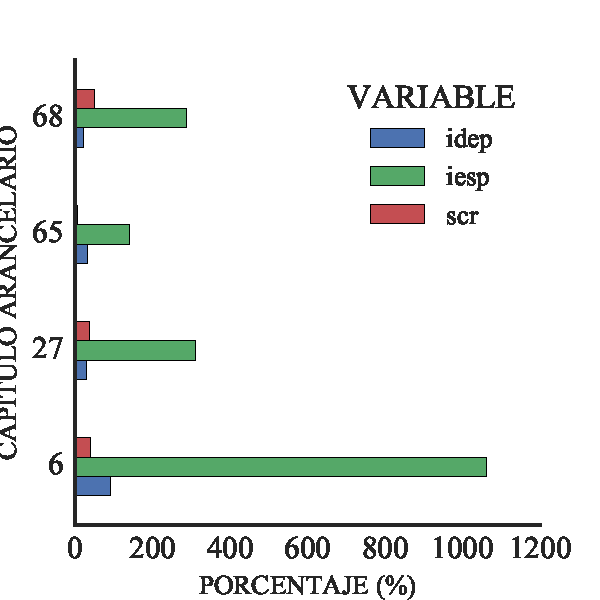
\includegraphics[width=250px]{esp_c2.pdf}
    \caption*{\textit{Fuente}: Elaboración propia con datos de \textit{PC-TAS}}
    \label{esp_c2}
\end{figure}

% cuadrante 3

\begin{table}[ht]
    \centering
    \caption{Cuadrante 3}
    \label{tab_c3}
    \resizebox{\textwidth}{!}{%
    \begin{tabular}{@{}lllllll@{}}
    \toprule
    & idep                                                                                                          & iesp   & scr      & irx     & irm   & igl   &       \\ \midrule
    Pescados y crustáceos, moluscos y demás invertebrados acuáticos                                               & 146,76 & 465,79   & -4,65   & 4,19  & 1,03  & 95,35 \\
    Hortalizas, plantas, raíces y tubérculos alimenticios                                                         & 100,05 & 410,83   & -23,23  & 1,94  & 0,70  & 76,77 \\
    Café, té, yerba mate y especias                                                                               & 486,01 & 0,00     & -100,00 & 0,00  & 1,93  & 0,00  \\
    Cacao y sus preparaciones                                                                                     & 148,51 & 344,54   & -31,82  & 1,53  & 0,67  & 68,18 \\
    Preparaciones de hortalizas, frutas u otros frutos o demás partes de plantas                                  & 261,89 & 58,27    & -85,23  & 0,66  & 1,87  & 14,77 \\
    Bebidas, líquidos alcohólicos y vinagre                                                                       & 471,69 & 1.009,57 & -32,35  & 3,53  & 1,55  & 67,65 \\
    Sal; azufre; tierras y piedras; yesos, cales y cementos                                                       & 157,01 & 263,79   & -72,73  & 17,79 & 25,28 & 27,27 \\
    Abonos                                                                                                        & 254,63 & 29,80    & -92,11  & 0,31  & 1,67  & 7,89  \\
    Madera, carbón vegetal y manufacturas de madera                                                               & 125,75 & 19,91    & -91,52  & 0,36  & 1,81  & 8,48  \\
    Guata, fieltro y tela sin tejer, hilados especiales; cordeles, cuerdas y cordajes; artículos de cordelería    & 124,37 & 36,79    & -92,45  & 0,31  & 1,75  & 7,55  \\
    Alfombras y demás revestimientos para el suelo, de materia textil                                             & 152,07 & 24,69    & -94,97  & 0,26  & 2,22  & 5,03  \\
    Plumas y plumón preparados y artículos de plumas o plumón; flores artificiales; manufacturas de cabello       & 102,22 & 42,95    & -78,29  & 0,97  & 1,79  & 21,71 \\
    Reactores nucleares, calderas, máquinas, aparatos y artefactos mecánicos; partes de estas máquinas o aparatos & 184,26 & 47,49    & -87,96  & 0,66  & 2,33  & 12,04 \\ \bottomrule
    \end{tabular}
    }
    \caption*{\textit{Fuente}: Elaboración propia con datos de \textit{PC-TAS}}
\end{table}

\begin{figure}[ht]
    \centering
    \caption{Indicadores de especialización comerciale por cuadrantes para cada sector}
    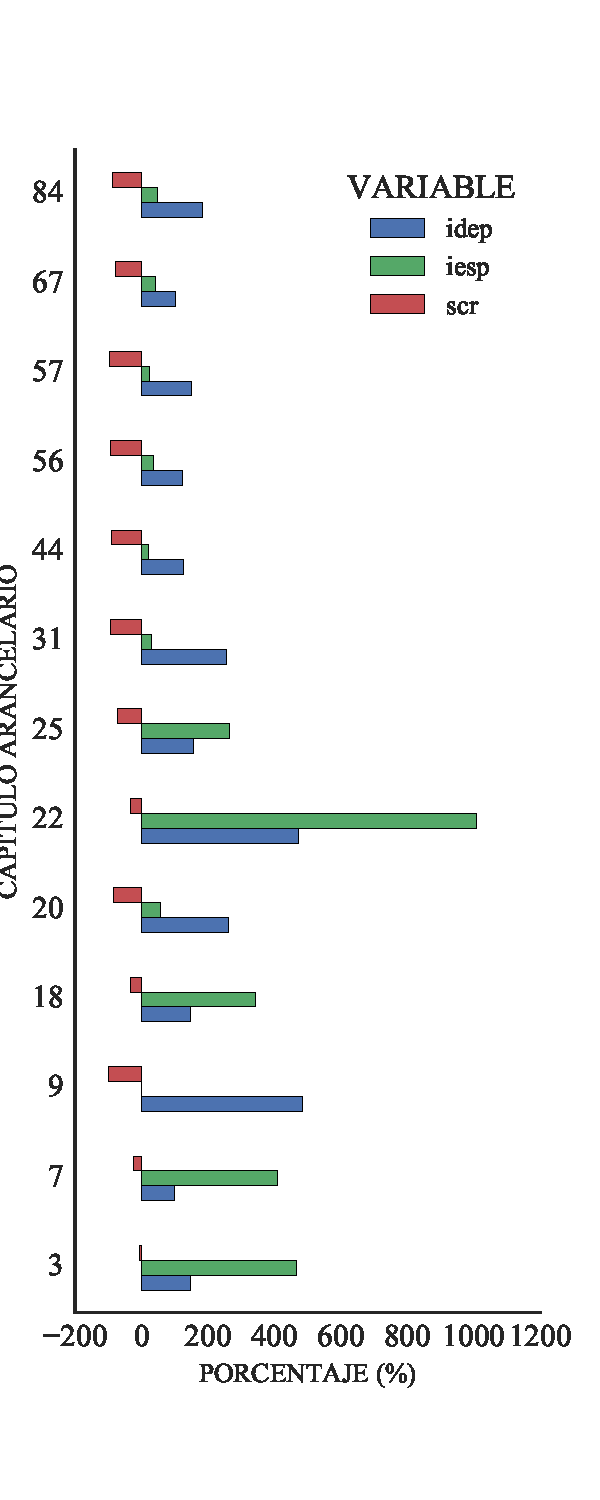
\includegraphics[width=250px]{esp_c3.pdf}
    \caption*{\textit{Fuente}: Elaboración propia con datos de \textit{PC-TAS}}
    \label{esp_c3}
\end{figure}


% cuadrante 4
\begin{table}[ht]
    \centering
    \caption{Cuadrante 4}
    \label{tab_c4}
    \resizebox{\textwidth}{!}{%
    \begin{tabular}{@{}lllllll@{}}
    \toprule
    & idep                                                                                                                                                          & iesp   & scr      & irx    & irm   & igl   &       \\ \midrule
    Pescados y crustáceos, moluscos y demás invertebrados acuáticos                                                                                               & 146,76 & 465,79   & -4,65  & 4,19  & 1,03  & 95,35 \\
    Hortalizas, plantas, raíces y tubérculos alimenticios                                                                                                         & 100,05 & 410,83   & -23,23 & 1,94  & 0,70  & 76,77 \\
    Cacao y sus preparaciones                                                                                                                                     & 148,51 & 344,54   & -31,82 & 1,53  & 0,67  & 68,18 \\
    Bebidas, líquidos alcohólicos y vinagre                                                                                                                       & 471,69 & 1.009,57 & -32,35 & 3,53  & 1,55  & 67,65 \\
    Sal; azufre; tierras y piedras; yesos, cales y cementos                                                                                                       & 157,01 & 263,79   & -72,73 & 17,79 & 25,28 & 27,27 \\
    Productos químicos inorgánicos; compuestos inorgánicos u orgánicos de metal precioso, de elementos radiactivos, de metales de las tierras raras o de isótopos & 88,85  & 277,71   & -3,60  & 14,37 & 3,46  & 96,40 \\
    Estaño y sus manufacturas                                                                                                                                     & 67,61  & 102,81   & -40,37 & 3,32  & 1,75  & 59,63 \\ \bottomrule
    \end{tabular}
    }
    \caption*{\textit{Fuente}: Elaboración propia con datos de \textit{PC-TAS}}
\end{table}

\begin{figure}[ht]
    \centering
    \caption{Indicadores de especialización comerciale por cuadrantes para cada sector}
    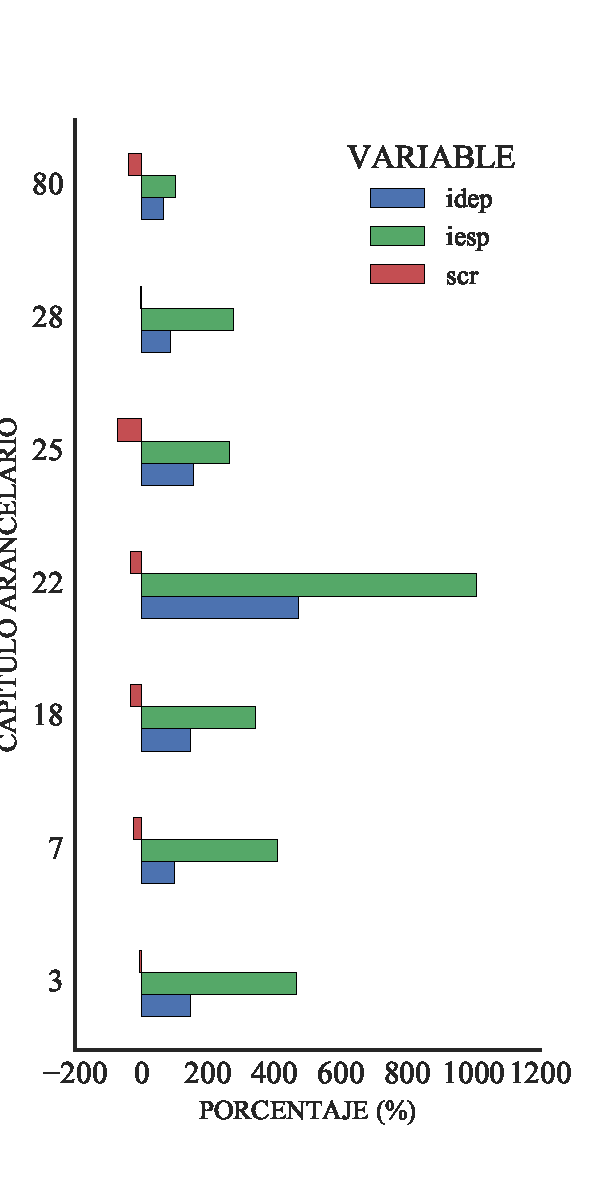
\includegraphics[width=250px]{esp_c4.pdf}
    \caption*{\textit{Fuente}: Elaboración propia con datos de \textit{PC-TAS}}
    \label{esp_c4}
\end{figure}

\chapter{Política Comercial}

El apartado de política comercial, Chipre no presenta datos actualizados individuales al pertenecer a la UE desde 2008, en su lugar adopta las mismas medidas que la UE en materia de comercio exterior.

Según el examen de políticas comerciales de la secretaria de la OMC Como Chipre tiene factores externos terminaste crecimiento lo que provoca una dependencia del país respecto de turismo además, tiene bajo nivel de inversión en maquinaria equipo. Chipre tiene déficit comercial estructural, las importaciones de mercancías representa cerca del 40\% del PIB. Las exportaciones de mercancías están igualmente repartidas entre productos de Agricultura y manufacturados.

La evolución reciente de Chipre en materia de política comercial, estuvo marcada por la adhesión en Unión Europea, la mayoría de aranceles son ad valorem, que principalmente afectan a productos agropecuarios. Además hay aranceles aplicación frontera. Se aplican prohibiciones de la importación para poner en práctica acuerdos de protección del medioambiente. Se ha reducido literal para cenar presiones inflacionarias. Chipre no tiene previsiones de exportación.

Chipre tiene en proceso de revisión su legislación antidumping. Sobre políticas comerciales sectoriales en la agricultura Chipre ofreció consolidar a tipos máximos de entre 30 y 245\%. El promedio aritmético de los aranceles de Chipre para productos de cultura en 1996 fue del 37,6\%. En el sector manufacturas, Chipre es importador neto, el país consolidó alrededor del 80\% de sus líneas arancelarias de productos industriales en el 40\%, aunque los tipos efectivos aplicados son muy inferiores, el promedio de los aranceles a los productos industriales fue del 10,9\%,  y para las importaciones provenientes de la Unión Europea del 3\%.

Para el sector servicios Chipre tiene establecido el máximo de participación extranjera en el capital el 49\% para las agencias de viajes organización de viajes en grupo y alquiler de automóviles. La reforma más importante fue la liberación financiera cambios legislativos en materia de blanqueo de dinero y fiscalización.

En cuanto al perfil arancelario de Chipre, adopta el mismo que la Unión Europea desde su adhesión en 2008, por lo cual, se analiza el perfil del mismo.

Según el informe de perfiles arancelarios en el mundo 2016, la Unión Europea (Y por tanto Chipre), tiene un NMF aplicado promedio para 2015 del 5,1\% para el total de productos, en los agropecuarios tiene un 10,7\%, Y para los no agropecuarios un 4,2\%. El promedio ponderado de aranceles para 2014 en el total de productos fue del 2,7\%, para los agropecuarios el 8,5\%, Y el 2,3\% para los no agropecuarios.

Por un grupo de productos los más importantes son el petróleo cuidas importaciones están exentas en un 98\%, Máquinas no eléctricas cuyas importaciones están exentas en los 56,7\% imaginas eléctricas exentas en un 63, 1\% cuantas exportaciones principales mercados son estados Unidos con aranceles en promedio de 7,1\%, Federación de Rusia en promedio 15,4\% Y China con un promedio del 15,2\%.

\chapter{Resumen y Conclusiones}

Chipre es un país con una gran riqueza, pero con ciertas taras políticas Y un gran potencial. De cara al exterior, la Introducción en la Unión Europea ha tenido una gran repercusión en la economía que se han reflejado en la mayoría de indicadores, por ejemplo en la relación real de intercambio, la evolución de las exportaciones importaciones, y los tipo de cambio.

Además, ha tenido que hacer un gran esfuerzo fiscal y macroeconómico en el proceso integración. En cuanto al comercio interindustrial los indicadores no puedes explicar el patrón de comercio los sectores mediante la ventaja comparativa, sin embargo todos los sectores siguen el patrón de comercio intraindustrial, por ejemplo, economía de escala, innovación, marketing, preferencias del consumidor.

En materia de política exterior, la integración de la Unión Europea ha propiciado cambios que materia arancelaria consolidarme o el 80\% de sus líneas arancelarias.

% ––––––––––––––––––––––––––––––– ANEXO –––––––––––––––––––––––––––––––––

\chapter{Anexo}
\pagestyle{empty}
\thispagestyle{empty}
En el Capítulo \ref{cap1} se han usado los siguientes indicadores:

\begin{enumerate}
    \item BALANZA COMERCIAL

    $$X - M$$
    \item TASA DE COBERTURA

    $$\frac{X}{M}100$$
    \item PENETRACIÓN DE LAS IMPORTACIONES

    $$\frac{M}{\text{PIB} + M - X} 100$$
    \item GRADO DE APERTURA

    $$\frac{X+M}{\text{PIB}} 100$$
    \item PROPENSIÓN EXPORTADORA

    $$\frac{X}{\text{PIB}} 100$$

\end{enumerate}

En el Capítulo \ref{cap3}:

\begin{enumerate}
    \item COMPETITIVIDAD PRECIO O COSTE
    \begin{enumerate}
        \item Indices de tipo de cambio efectivo real
        \item Tipo de cambio oficial
        \item Tasa de inflación
    \end{enumerate}

    \item ESPECIALIZACIÓN COMERCIAL

    \item  INDICE DE DEPENDENCIA

    Para todo país $h$ y el sector $i$

    $$IDep^h_i = \frac{\frac{M^h_i}{\sum_i M^h_i}}{\frac{\sum_h M^h_i}{\sum_h \sum_i M^h_i}} 100$$

    \item  INDICE DE ESPECIALIZACIÓN

    $$IEsp^h_i = \frac{\frac{X^h_i}{\sum_i X^h_i}}{\frac{\sum_h X^h_i}{\sum_h \sum_i X^h_i}} 100$$

    \item  SALDO COMERCIAL RELATIVO

    $$SCR_i = \frac{X_i - M_i}{X_i + M_i} 100$$

    \item IMPORTANCIA RELATIVA DEL SECTOR EN LAS IMPORTACIONES Y EXPORTACIONES.

    $$IRX_i = \frac{X_i}{\sum_i X_i}$$

    $$IRM_i = \frac{M_i}{\sum_i M_i}$$

    \item COMERCIO INTRAINDUSTRIAL

    $$IGL_i = \frac{X_i + M_i - |X_i - M_i|}{X_i + M_i}100$$

    $$IGL_{agg} = \frac{\sum_i(X_i + M_i) - \sum_i |X_i - M_i|}{\sum_i (X_i + M_i)}100$$

\end{enumerate}

En el Capítulo \ref{cap6}:

\begin{enumerate}

    \item INDICE DE DEPENDENCIA

    Para todo país $h$ y el sector $i$

    \begin{equation}
    IDep^h_i = \frac{\frac{M^h_i}{\sum_i M^h_i}}{\frac{\sum_h M^h_i}{\sum_h \sum_i M^h_i}} 100
    \end{equation}

    \item INDICE DE ESPECIALIZACIÓN

    \begin{equation}
    IEsp^h_i = \frac{\frac{X^h_i}{\sum_i X^h_i}}{\frac{\sum_h X^h_i}{\sum_h \sum_i X^h_i}} 100
    \end{equation}

    \item SALDO COMERCIAL RELATIVO

    \begin{equation}
    SCR_i = \frac{X_i - M_i}{X_i + M_i} 100
    \end{equation}

    \item IMPORTANCIA RELATIVA DEL SECTOR EN LAS IMPORTACIONES Y EXPORTACIONES.

    \begin{equation}
    IRX_i = \frac{X_i}{\sum_i X_i}
    \end{equation}

    \begin{equation}
    IRM_i = \frac{M_i}{\sum_i M_i}
    \end{equation}

\end{enumerate}

\subsection{Capítulos Arancelarios}

\begin{table}[]
    \centering
    \caption{Capítulos arancelarios}
    \label{arm}
    \resizebox{\textwidth}{!}{%
    \begin{tabular}{@{}ll@{}}
    \toprule
    cod & descripción                                                                                                                                                                                                                                                                                    \\ \midrule
    1   & Animales vivos                                                                                                                                                                                                                                                                                 \\
    2   & Carne y Despojos Comestibles                                                                                                                                                                                                                                                                   \\
    3   & Pescados y crustáceos, moluscos y demás invertebrados acuáticos                                                                                                                                                                                                                                \\
    4   & Leche y productos lácteos; huevos de ave; miel natural; productos comestibles de origen animal, no expresados ni comprendidos en otra parte                                                                                                                                                    \\
    5   & Los demás productos de origen animal, no expresados ni comprendidos en otra parte                                                                                                                                                                                                              \\
    6   & Plantas vivas y productos de la floricultura                                                                                                                                                                                                                                                   \\
    7   & Hortalizas, plantas, raíces y tubérculos alimenticios                                                                                                                                                                                                                                          \\
    8   & Frutas y frutos comestibles; cortezas de agrios (cítricos), melones o sandías                                                                                                                                                                                                                  \\
    9   & Café, té, yerba mate y especias                                                                                                                                                                                                                                                                \\
    10  & Cereales .                                                                                                                                                                                                                                                                                     \\
    11  & Productos de la molinería; malta; almidón y fécula; inulina; gluten de trigo                                                                                                                                                                                                                   \\
    12  & Semillas y frutos oleaginosos; semillas y frutos diversos; plantas industriales o medicinales; paja y forraje                                                                                                                                                                                  \\
    13  & Gomas, resinas y demás jugos y extractos vegetales                                                                                                                                                                                                                                             \\
    14  & Materias trenzables y demás productos de origen vegetal, no expresados ni comprendidos en otra parte                                                                                                                                                                                           \\
    15  & Grasas y aceites animales o vegetales; productos de su desdoblamiento; grasas alimenticias elaboradas;ceras de origen animal o vegetal                                                                                                                                                         \\
    16  & Preparaciones de carne, pescado o de crustáceos, moluscos o demás invertebrados acuáticos                                                                                                                                                                                                      \\
    17  & Azúcares y artículos de confitería                                                                                                                                                                                                                                                             \\
    18  & Cacao y sus preparaciones                                                                                                                                                                                                                                                                      \\
    19  & Preparaciones a base de cereales, harina, almidón, fécula o leche; productos de pastelería                                                                                                                                                                                                     \\
    20  & Preparaciones de hortalizas, frutas u otros frutos o demás partes de plantas                                                                                                                                                                                                                   \\
    21  & Preparaciones alimenticias diversas                                                                                                                                                                                                                                                            \\
    22  & Bebidas, líquidos alcohólicos y vinagre                                                                                                                                                                                                                                                        \\
    23  & Residuos y desperdicios de las industrias alimentarias; alimentos preparados para animales                                                                                                                                                                                                     \\
    24  & Tabaco y sucedáneos del tabaco, elaborados                                                                                                                                                                                                                                                     \\
    25  & Sal; azufre; tierras y piedras; yesos, cales y cementos                                                                                                                                                                                                                                        \\
    26  & Minerales metalíferos, escorias y cenizas                                                                                                                                                                                                                                                      \\
    27  & Combustibles minerales, aceites minerales y productos de su destilación; materias bituminosas;ceras minerales                                                                                                                                                                                  \\
    28  & Productos químicos inorgánicos; compuestos inorgánicos u orgánicos de metal precioso, de elementos radiactivos, de metales de las tierras raras o de isótopos                                                                                                                                  \\
    29  & Productos químicos orgánicos                                                                                                                                                                                                                                                                   \\
    30  & Productos farmacéuticos                                                                                                                                                                                                                                                                        \\
    31  & Abonos                                                                                                                                                                                                                                                                                         \\
    32  & Extractos curtientes o tintóreos; taninos y sus derivados; pigmentos y demás materias colorantes; pinturas y barnices; mástiques; tintas                                                                                                                                                       \\
    33  & Aceites esenciales y resinoides; preparaciones de perfumería, tocador o cosmética                                                                                                                                                                                                              \\
    34  & Jabón, agentes de superficie orgánicos, preparaciones para lavar, preparaciones lubricantes, ceras artificiales, ceras preparadas, productos de limpieza, velas y artículos similares, pastas para modelar, “ceras para odontología” y preparaciones para odontología a base de yeso fraguable \\
    35  & Materias albuminóideas; productos a base de almidón o de fécula modificados;colas; enzimas                                                                                                                                                                                                     \\
    36  & Pólvora y explosivos; artículos de pirotecnia; fósforos (cerillas); aleaciones pirofóricas; materias inflamables                                                                                                                                                                               \\
    37  & Productos fotográficos o cinematográficos                                                                                                                                                                                                                                                      \\
    38  & Productos diversos de las industrias químicas                                                                                                                                                                                                                                                  \\
    39  & Plástico y sus manufacturas                                                                                                                                                                                                                                                                    \\
    40  & Caucho sus manufacturas                                                                                                                                                                                                                                                                        \\
    41  & Pieles (excepto la peletería) y cueros                                                                                                                                                                                                                                                         \\
    42  & Manufacturas de cuero; artículos de talabartería o guarnicionería; artículos de viaje, bolsos de mano (carteras) y continentes similares; manufacturas de tripa                                                                                                                                \\
    43  & Peletería y confecciones de peletería; peletería facticia o artificial                                                                                                                                                                                                                         \\
    44  & Madera, carbón vegetal y manufacturas de madera                                                                                                                                                                                                                                                \\
    45  & Corcho y sus manufacturas                                                                                                                                                                                                                                                                      \\
    46  & Manufacturas de espartería o cestería                                                                                                                                                                                                                                                          \\
    47  & Pasta de Madera o de las demás materias fibrosas celulósicas; papel o cartón para reciclar (desperdicios y desechos)                                                                                                                                                                           \\
    48  & Papel y cartón; manufacturas de pasta de celulosa, de papel o cartón                                                                                                                                                                                                                           \\
    49  & Productos editoriales de la prensa y de las demás industrias gráficas; textos manuscritos o mecanografiados y planos                                                                                                                                                                           \\
    50  & Seda                                                                                                                                                                                                                                                                                           \\
    51  & Lana y pelo fino u ordinario; hilados y tejidos de crin                                                                                                                                                                                                                                        \\
    52  & Algodón                                                                                                                                                                                                                                                                                        \\
    53  & Las demás fibras textiles vegetales; hilados de papel y tejidos de hilados de papel                                                                                                                                                                                                            \\
    54  & Filamentos sintéticos o artificiales                                                                                                                                                                                                                                                           \\
    55  & Fibras sintéticas o artificiales discontinuas                                                                                                                                                                                                                                                  \\
    56  & Guata, fieltro y tela sin tejer, hilados especiales; cordeles, cuerdas y cordajes; artículos de cordelería                                                                                                                                                                                     \\
    57  & Alfombras y demás revestimientos para el suelo, de materia textil                                                                                                                                                                                                                              \\
    58  & Tejidos especiales; superficies textiles con mechón insertado; encajes; tapicería; pasamanería; bordados                                                                                                                                                                                       \\
    59  & Telas impregnadas, recubiertas, revestidas o estratificadas; artículos técnicos de materia textil                                                                                                                                                                                              \\
    60  & Tejidos de punto                                                                                                                                                                                                                                                                               \\
    61  & Prendas y complementos (accesorios), de vestir, de punto                                                                                                                                                                                                                                       \\
    62  & Prendas y complementos (accesorios), de vestir, excepto los de punto                                                                                                                                                                                                                           \\
    63  & Los demás artículos textiles confeccionados; juegos prendería y trapos                                                                                                                                                                                                                         \\
    64  & Calzado, polainas y artículos análogos; partes de estos artículos                                                                                                                                                                                                                              \\
    65  & Sombreros, demás tocados y sus partes.                                                                                                                                                                                                                                                         \\
    66  & Paraguas, sombrillas, quitasoles, bastones, bastones asiento, látigos, fustas y sus partes                                                                                                                                                                                                     \\
    67  & Plumas y plumón preparados y artículos de plumas o plumón; flores artificiales; manufacturas de cabello                                                                                                                                                                                        \\
    68  & Manufacturas de piedra, yeso fraguable, cemento, amianto (asbesto), mica o materias análogas                                                                                                                                                                                                   \\
    69  & Productos cerámicos                                                                                                                                                                                                                                                                            \\
    70  & Vidrio y sus manufacturas                                                                                                                                                                                                                                                                      \\
    71  & Perlas finas (naturales)* o cultivadas, piedras preciosas o semipreciosas, metales preciosos, electromecánicos) de señalización para vías de comunicación                                                                                                                                      \\
    72  & Fundición, hierro y acero .                                                                                                                                                                                                                                                                    \\
    73  & Manufacturas de fundición, hierro o acero                                                                                                                                                                                                                                                      \\
    74  & Cobre y sus manufacturas                                                                                                                                                                                                                                                                       \\
    75  & Níquel y sus manufacturas                                                                                                                                                                                                                                                                      \\
    76  & Aluminio y sus manufacturas                                                                                                                                                                                                                                                                    \\
    77  & (Reservado para una futura utilización en el Sistema Armonizado)                                                                                                                                                                                                                               \\
    78  & Plomo y sus manufacturas                                                                                                                                                                                                                                                                       \\
    79  & Cinc y sus manufacturas                                                                                                                                                                                                                                                                        \\
    80  & Estaño y sus manufacturas                                                                                                                                                                                                                                                                      \\
    81  & Los demás metales comunes; cermets; manufacturas de estas materias                                                                                                                                                                                                                             \\
    82  & Herramientas y útiles, artículos de cuchillería y cubiertos de mesa, de metal común; partes de estos artículos, de metal común                                                                                                                                                                 \\
    83  & Manufacturas diversas de metal común                                                                                                                                                                                                                                                           \\
    84  & Reactores nucleares, calderas, máquinas, aparatos y artefactos mecánicos; partes de estas máquinas o aparatos                                                                                                                                                                                  \\
    85  & Máquinas, aparatos y material eléctrico, y sus partes; aparatos de grabación o reproducción de sonido, aparatos de grabación o reproducción de imagen y sonido en televisión, y las partes y accesorios de estos aparatos.                                                                     \\
    86  & Vehículos y material para vías férreas o similares, y sus partes; aparatos mecánicos (incluso electromecánicos) de señalización para vías de comunicación                                                                                                                                      \\
    87  & Vehículos automóviles, tractores, velocípedos y demás vehículos terrestres; sus partes y accesorios                                                                                                                                                                                            \\
    88  & Aeronaves, vehículos espaciales y sus partes                                                                                                                                                                                                                                                   \\
    89  & Barcos y demás artefactos flotantes                                                                                                                                                                                                                                                            \\
    90  & Instrumentos y aparatos de óptica. fotografía o cinematografía, de medida, control o precisión; instrumentos y aparatos medicoquirúrgicos; partes y accesorios de estos instrumentos o aparatos                                                                                                \\
    91  & Aparatos de relojería y sus partes                                                                                                                                                                                                                                                             \\
    92  & Instrumentos musicales; sus partes y accesorios                                                                                                                                                                                                                                                \\
    93  & Armas, municiones, y sus partes y accesorios                                                                                                                                                                                                                                                   \\
    94  & Muebles; mobiliario medicoquirúrgico; artículos de cama y similares; aparatos de alumbrado no expresados ni comprendidos en otra parte; anuncios, letreros y placas indicadoras luminosos y artículos similares; construcciones prefabricadas                                                  \\
    95  & Juguetes, juegos y artículos para recreo o deporte; sus partes y accesorios                                                                                                                                                                                                                    \\
    96  & Manufacturas diversas de metal común                                                                                                                                                                                                                                                           \\
    97  & Objetos de arte o colección y antigüedades                                                                                                                                                                                                                                                     \\
    98  & (Reservado para usos particulares por las Partes Contratantes)                                                                                                                                                                                                                                 \\
    99  & (Reservado para usos particulares por las Partes Contratantes)                                                                                                                                                                                                                                 \\
    0   & Tratamientos arancelarios especiales                                                                                                                                                                                                                                                           \\ \bottomrule
    \end{tabular}%
    }
\end{table}


\cleardoublepage
\addcontentsline{toc}{chapter}{Bibliografía}
\bibliographystyle{apalike}
\bibliography{biblio} % yyyy.bib es el fichero donde está salvada la bibliografía.

\end{document}
